\chapter{State of the Art}
\markboth{State of the Art}{State of the Art}
\label{chapter:StateOfTheArt}


%%%%%%%%%%%%%%%%%%%%%%%%%%%%%%%%%%%%%%%%%%%%%%%%%%%%%%%%%%%%%%%%%%%%%%%%%%%%%%%%%%%%%%%%%%%%%%%%%%%%%%%%%%%%%%%%%%%%

In this section, we provide a state of the art on the synthesis of music performances, focusing on all the protagonists that act and are in interaction during an instrumental situation. It includes the modeling and animation of a virtual character, as well as its interaction with sound synthesis processes.\\

We draw an overview of the main virtual human models as well as the animation techniques that steer such representations to a desired motion (\emph{Computer Animation}, section \ref{sec:CA}).\\

We focus on the concepts that have been elaborated for synthesizing sounds, and specifically how these models are related to instrumental gestures (\emph{Computer Music}, section \ref{sec:CM}).\\

Although \emph{Computer Animation} and \emph{Computer Music} research fields have grown quite independantly along the years, we refer to works that can be considered at the frontier of these areas (section \ref{sec:SMP}). It includes an overview of various models for synthesizing real/virtual music performances, which is the core subject of our contributions.

%%%%%%%%%%%%%%%%%%%%%%%%%%%%%%%%%%%%%%%%%%%%%%%%%%%%%%%%%%%%%%%%%%%%%%%%%%%%%%%%%%%%%%%%%%%%%%%%%%%%%%%%%%%%%%%%%%%%


%%%%%%%%%%%%%%%%%%%%%%%%%%%%%%%%%%%%%%%%%%%%%%%%%%%%%%%%%%%%%%%%%%%%%%%%%%%%%%%%%%%%%%%%%%%%%%%%%%%%%%%%%%%%%%%%%%%%

	\section{Computer Animation}
	\label{sec:CA}

Nowadays, the exploration of virtual environments by virtual characters is a widespread issue in many applications. To cite a few, it ranges from video games to the film industry, as well as human movement analysis and perception. Whatever application is targetted, a virtual character model and animation technique has to be chosen, depending on the final application.\\

The \emph{Computer Animation} community commonly divides this problem into two stages: 1) provide a model (or representation) of the virtual character itself (subsection \ref{subsec:CA_VCM}), and 2) develop techniques for controlling this representation as wanted over time (subsection \ref{subsec:CA_MC}).


		\subsection{Virtual Character Models}
		\label{subsec:CA_VCM}
		
Many virtual character models have been proposed in the literature, but each has obviously been highly inspired by the human anatomy. A common basis for modeling the human anatomy is to consider a set of virtual limbs connected by virtual joints. It generally involves a hierachical tree structure (an example is provided in \myfigname \ref{fig:kinDyn3}) describing the dependencies between these virtual entities. Typically, two main representations are used in \emph{Computer Animation}, the kinematics-based and the physics-based representations.

\begin{figure}
	\begin{center}
		\subfigure[]{\label{fig:kinDyn1}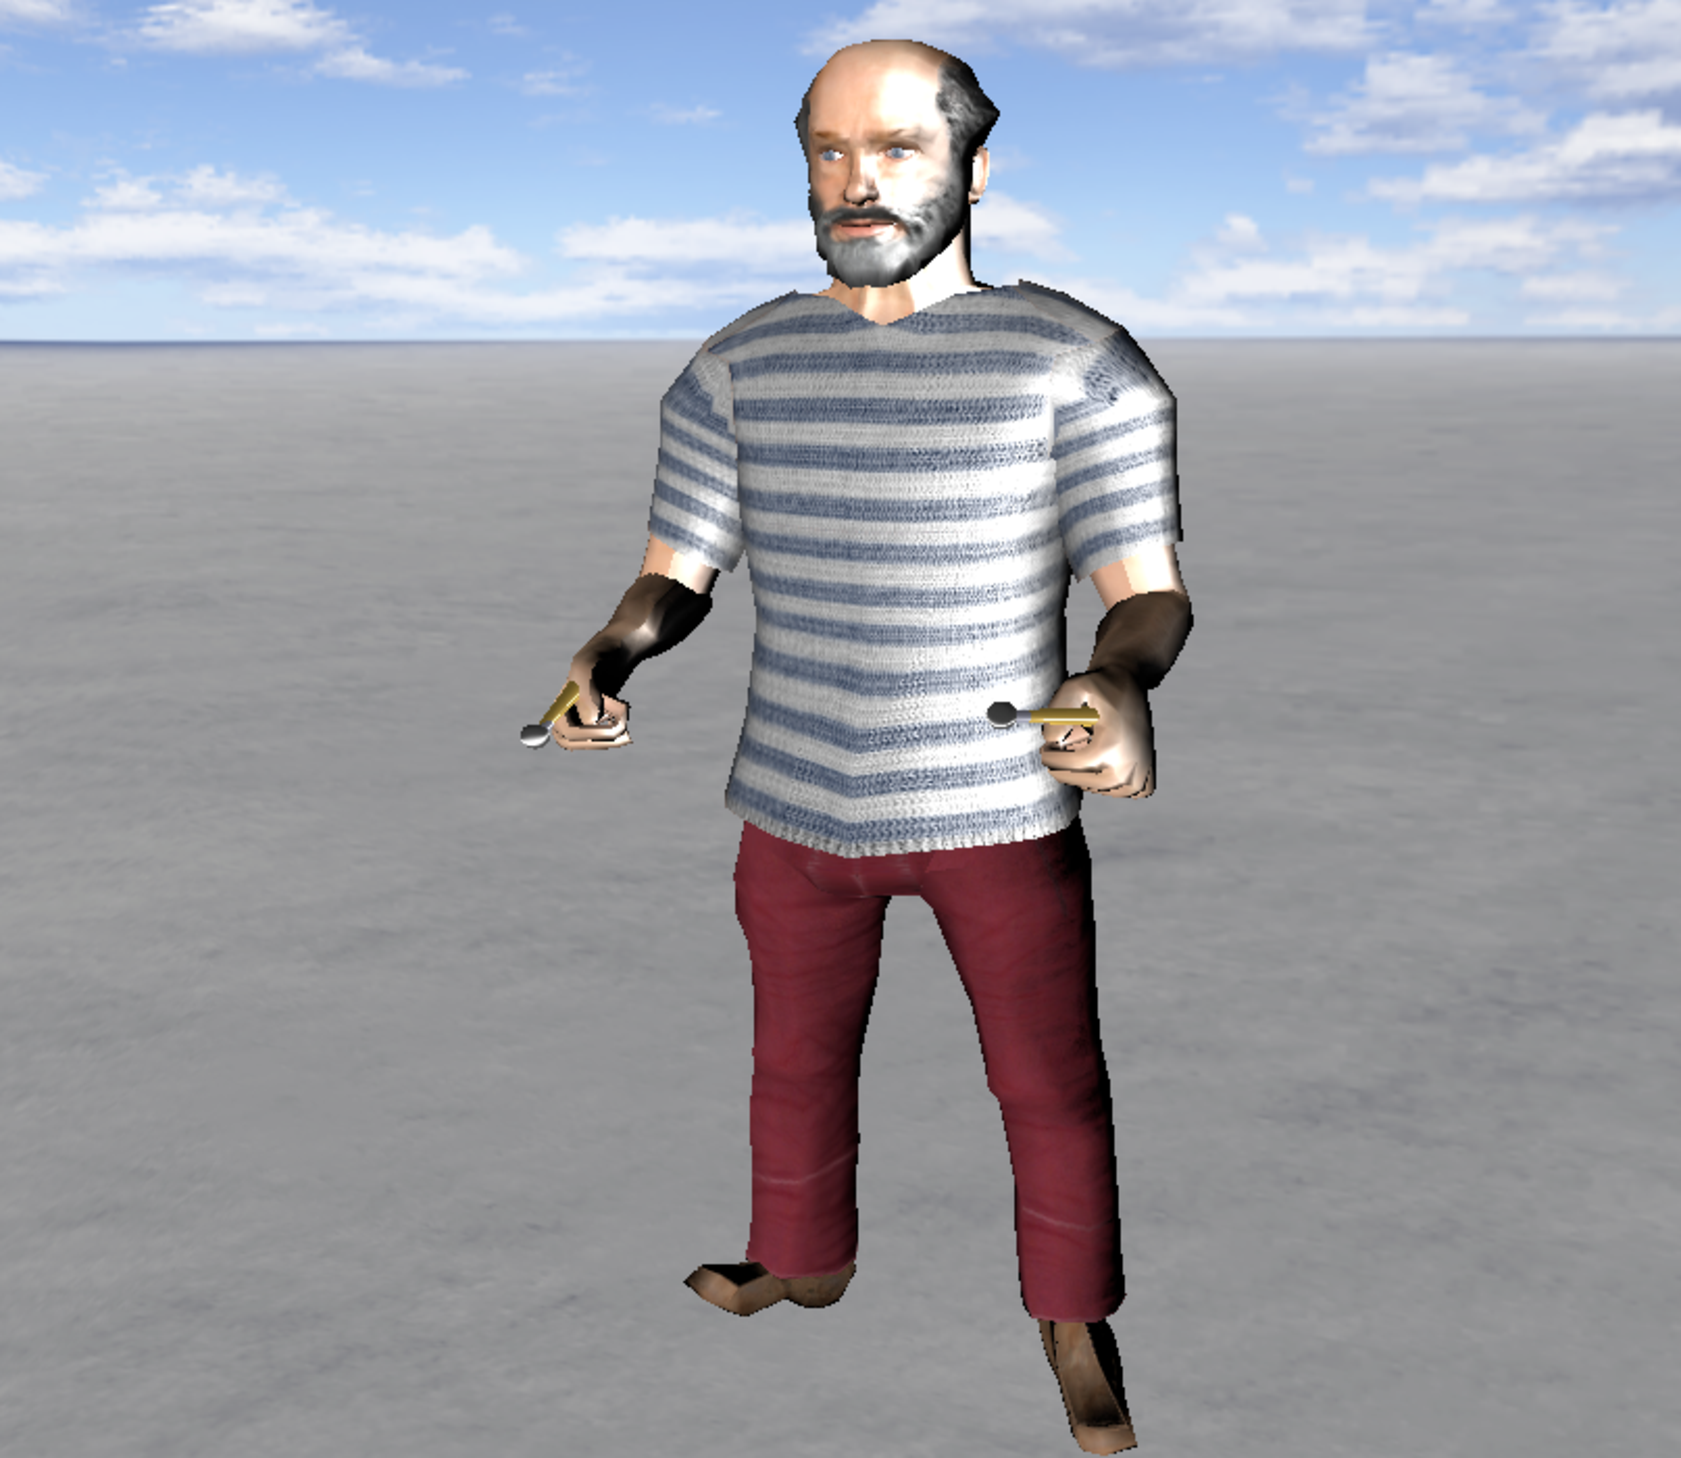
\includegraphics[width=0.48\columnwidth]{Chapters/2/Pics/Pdf/KinDyn1.pdf}}
		\subfigure[]{\label{fig:kinDyn3}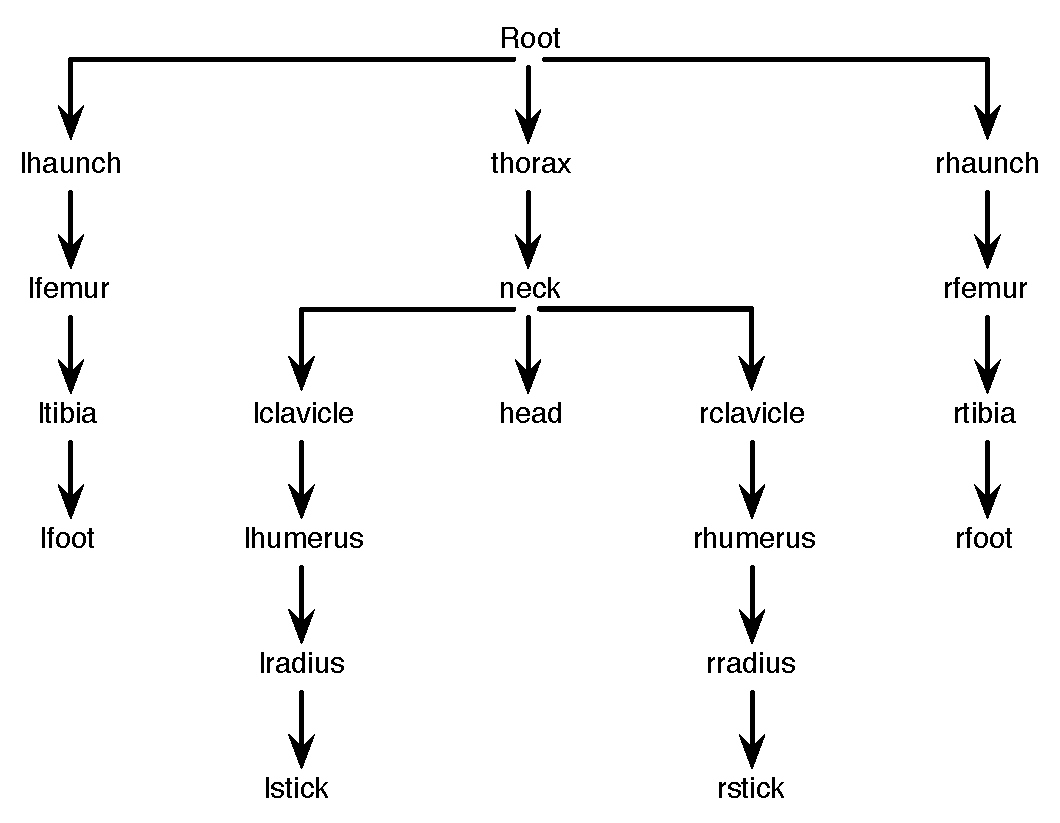
\includegraphics[width=0.48\columnwidth]{Chapters/2/Pics/Pdf/Kin.pdf}}
		\subfigure[]{\label{fig:kinDyn2}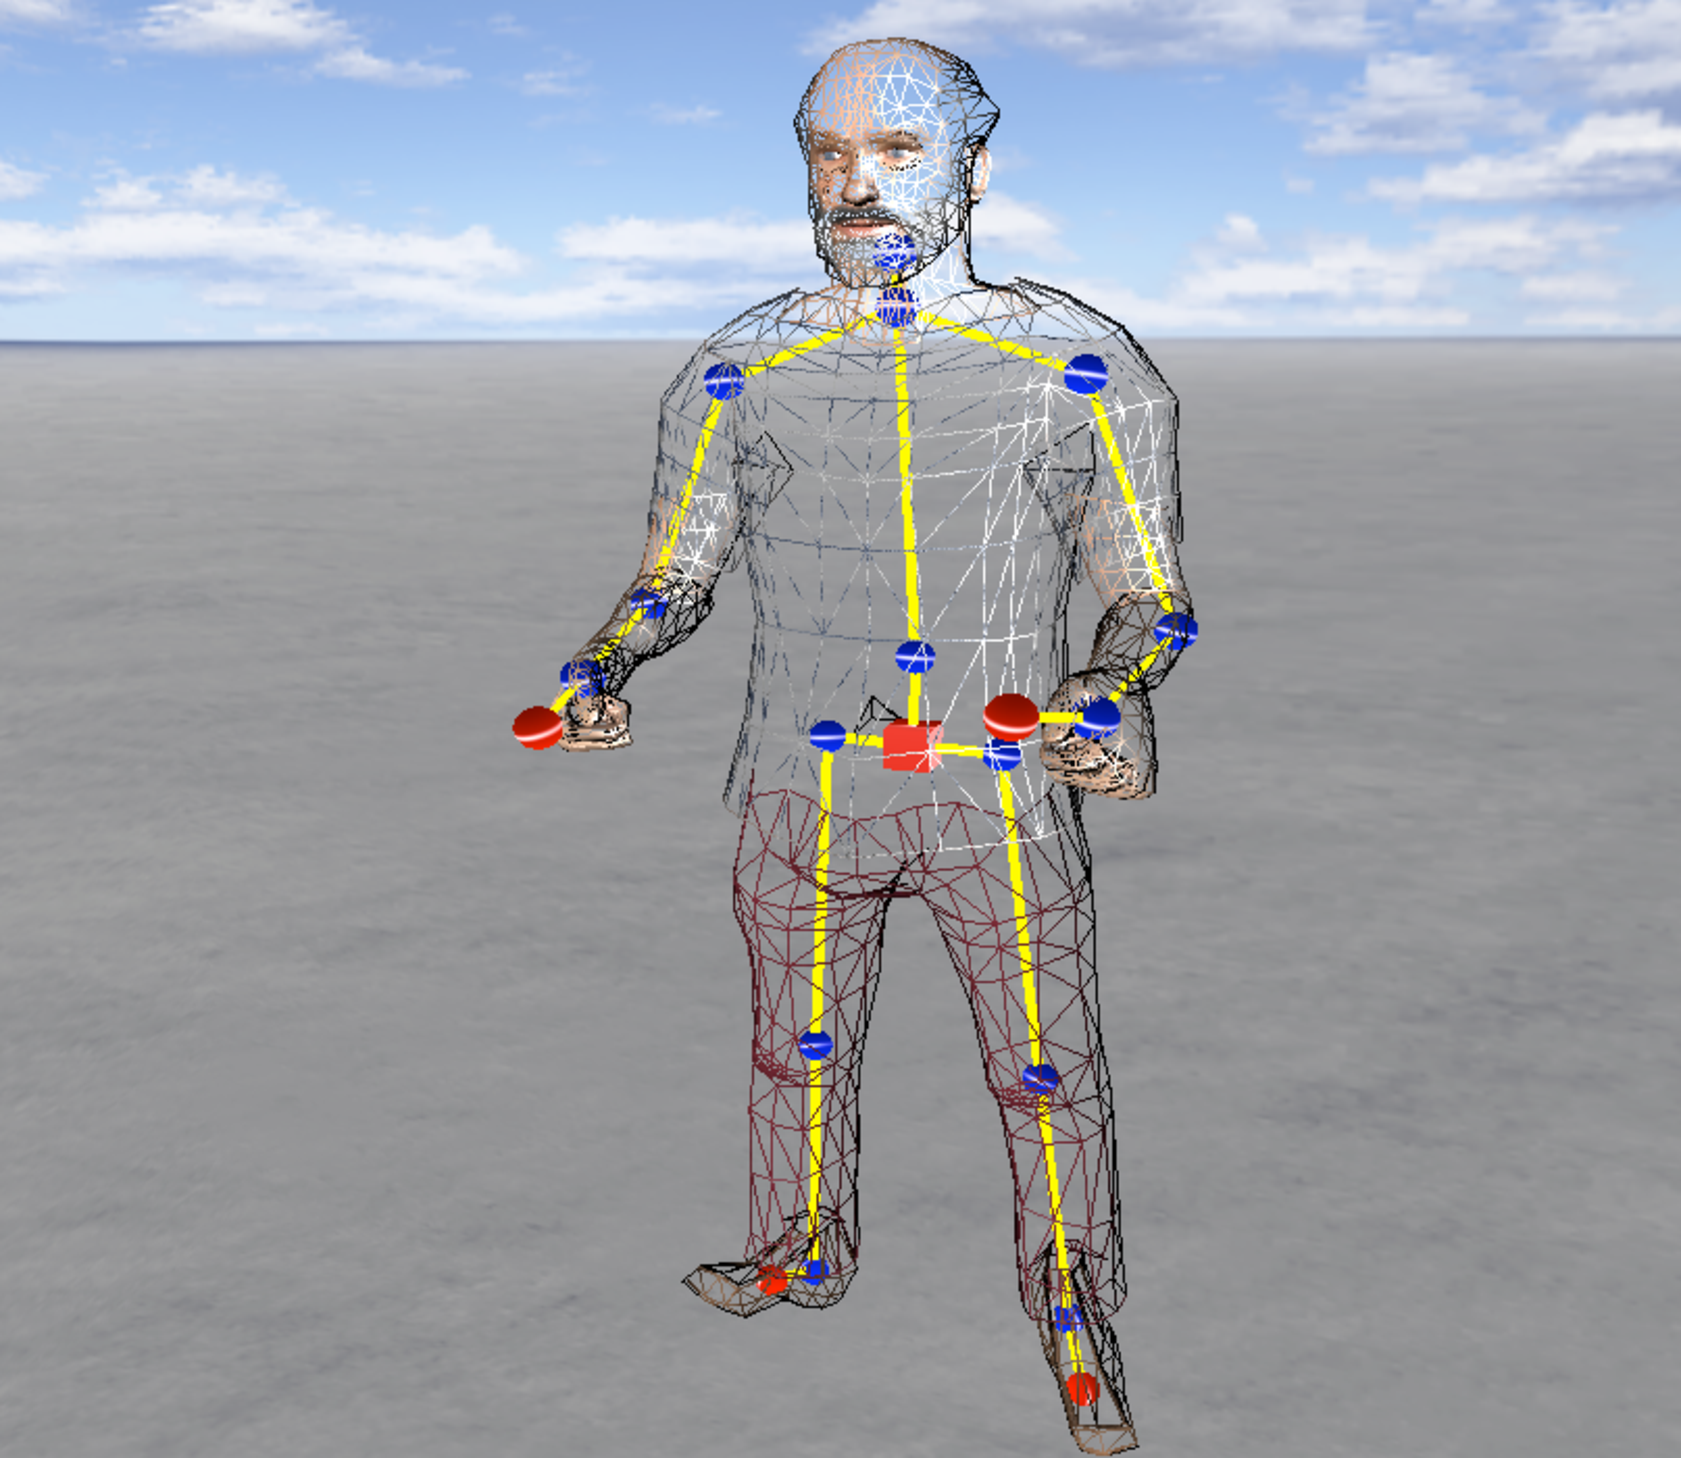
\includegraphics[width=0.48\columnwidth]{Chapters/2/Pics/Pdf/KinDyn2.pdf}}
		\subfigure[]{\label{fig:kinDyn4}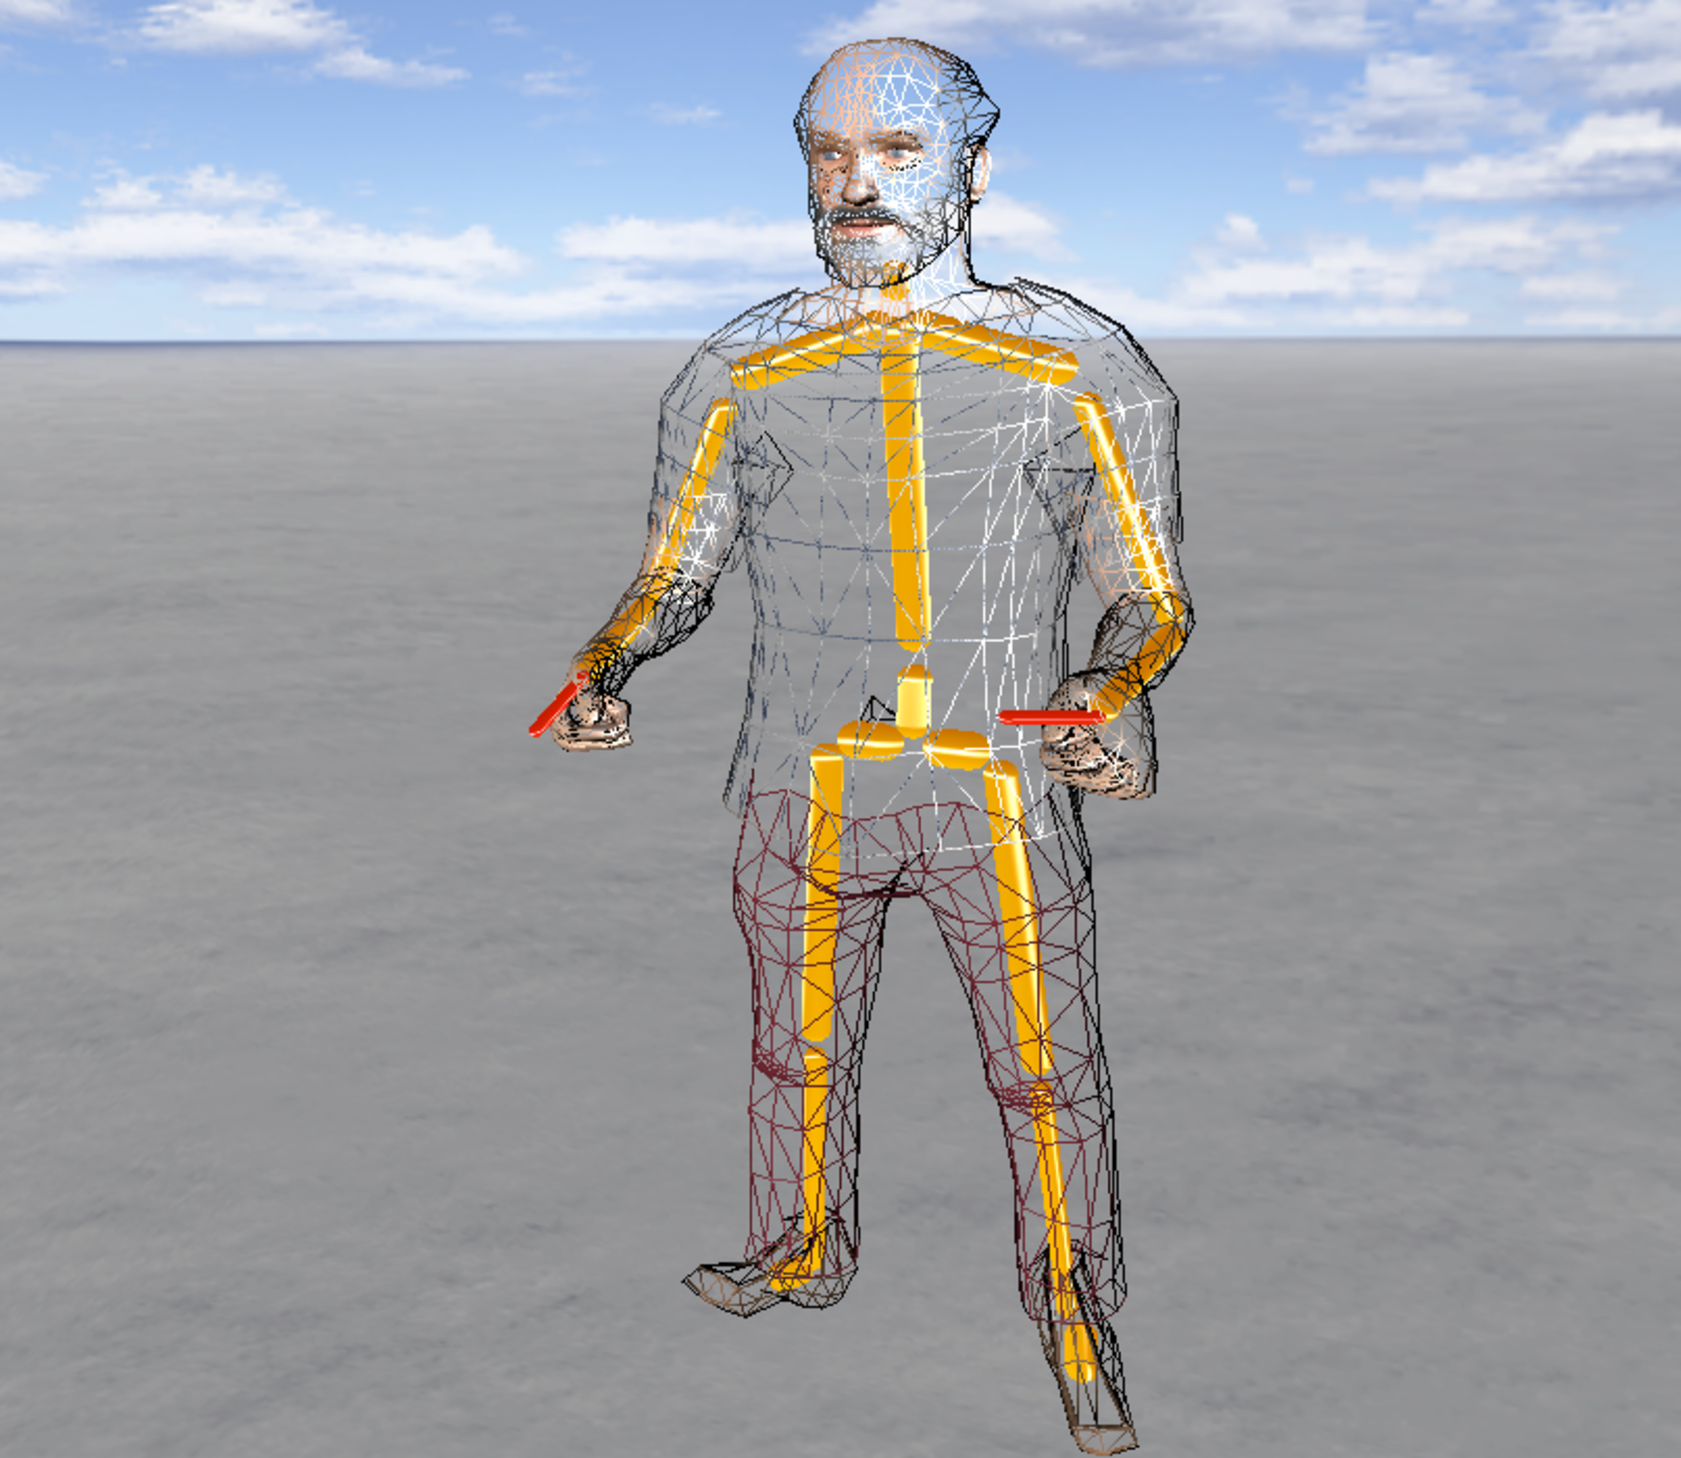
\includegraphics[width=0.48\columnwidth]{Chapters/2/Pics/Pdf/KinDyn4.pdf}}
	\end{center}
	\vspace{-0.5cm}
	\caption[Kinematics and physics representations of a virtual character]{Kinematics and physics representations of a virtual character: (a) final virtual character, (b) the hierachical tree structure, (c) an example of an underlying kinematic representation with its root (red box), set of joints (spheres) and implicit limbs (yellow lines), (d) an example of an underlying physic representation with its explicit limbs (capsule-shaped rigid bodies).}
	\label{fig:kinDynModels}
\end{figure}


			\subsubsection{Kinematics-based Representation}
			\label{subsubsec:CA_VCM_Kinematic}

Virtual characters can be represented by a \emph{kinematic} representation $\boldsymbol{T^K}$, which gives mainly a \emph{geometrical} interpretation of the human anatomy. Such a representation defines implicitly the limbs (or bones) of the virtual human by segments between paired joints. This hiearchical structure is defined by a root joint $\boldsymbol{j^K_r}$ (usually the pelvis) and a set of child joints $\boldsymbol{j^K}$, \myequname \eqref{eq:kinRepresentation}.\\

The kinematic system $\boldsymbol{T^K}$ is then defined by the observation of its state over time, \emph{i.e.} a kinematic configuration (or \emph{pose}) $\boldsymbol{q^K}$. $\boldsymbol{q^K}$ is composed of the root joint position $\boldsymbol{r}$ and the angular state of each child joint $\boldsymbol{\Theta^K}$, \myequname \eqref{eq:kinConfiguration}. The latter may have several \emph{degrees of freedom} (or \emph{DoFs}), thus constraining the motion of the virtual character.

\begin{equation}
	\boldsymbol{T^K} = [\boldsymbol{j^K_r}, \boldsymbol{j^K} = \lbrace j^K_i\rbrace_{i \in [1 \dots n]}]
\label{eq:kinRepresentation}
\eqcaption{Virtual character kinematic representation}
\end{equation}

\vspace{-0.4cm}

\begin{equation}
	\boldsymbol{q^K} = [\textbf{r}, \boldsymbol{\Theta^K} = \lbrace \Theta^K_i\rbrace_{i \in [1 \dots n]}]
\label{eq:kinConfiguration}
\eqcaption{Virtual character kinematic configuration}
\end{equation}

\myfigname \ref{fig:kinDyn2} depicts an example of kinematic representation of a virtual character, with its root position (red box), set of joints (spheres) and implicit limbs (yellow lines). A standard kinematic representation for modeling virtual characters is commonly used for this type of approach \citeCGA{hanim}, easying the comparison, sharing and reusability of representations.


			\subsubsection{Physics-based Representation}
			\label{subsubsec:CA_VCM_Physic}

The \emph{physical} representation $\boldsymbol{T^D}$ of a virtual character provides a \emph{dynamic} interpretation of the human anatomy. In this case, the bones are explicitly modeled by a set of rigid solids $\boldsymbol{s^D}$ articulated by mechanical joints $\boldsymbol{j^D}$, \myequname \eqref{eq:dynRepresentation}. Every solid composing this physical representation $\boldsymbol{s^D}$ is parameterized by physical characteristics such as its mass \emph{m}, density \emph{d} and inertia tensor \emph{I}. Mechanical joints $\boldsymbol{j^D}$ can also be characterized by several DoFs constraining the motion, as well as physical features influencing the relative behavior between solids at the joint level.\\

The observation of the state of $\boldsymbol{T^D}$ over time leads to a dynamic configuration $\boldsymbol{q^D}$, composed of each rigid body linear-angular position $\boldsymbol{r^D}$ as well as each mechanical joint angular position $\boldsymbol{\Theta^D}$, \myequname \eqref{eq:dynConfiguration}. 

\begin{equation}
	\boldsymbol{T^D} = [\boldsymbol{s^D} = \lbrace m^D_i, d^D_i, I^D_i\rbrace_{i \in [1 \dots n]}, \boldsymbol{j^D} = \lbrace k^D_{s, j}, k^D_{d, j}\rbrace_{j \in [1 \dots m]}]
\label{eq:dynRepresentation}
\eqcaption{Virtual character dynamic representation}
\end{equation}

\vspace{-0.4cm}

\begin{equation}
	\boldsymbol{q^D} = [\boldsymbol{r^D} = \lbrace r^D_i, \Theta^D_{r, i}\rbrace_{i \in [1 \dots n]}, \boldsymbol{\Theta^D} = \lbrace \Theta^D_j\rbrace_{j \in [1 \dots m]}]
\label{eq:dynConfiguration}
\eqcaption{Virtual character dynamic configuration}
\end{equation}

\myfigname \ref{fig:kinDyn4} shows an example of a physic representation of a virtual character made of capsule-shaped rigid bodies. These models usually assume a uniform density distribution of the rigid bodies. Human body measures can be considered for initializing the physical properties of the rigid bodies composing such a representation \citeCGA{dempster:AJA67, AIST}.


		\subsection{Motion Control of Virtual Characters}
		\label{subsec:CA_MC}

The characteristics of these different virtual character representations previously presented intrinsically differ from the nature of human motion features they focus on. They differ as well as on the low/high level control properties and environment interactions that they can take into account.\\

The \emph{kinematic} model can be considered as an \emph{effect-centered} representation, offering a well formulated formalism for a high task control level. It however provides no explanation of the causes that are at the origin of the motion system $\boldsymbol{T^S}$, and harldy provides the opportunity to integrate interactions with its surrounding environment. Kinematics-based animation techniques will therefore use methods on the top of the geometrical observation $\boldsymbol{q^K}$ of the human motion, in order to reproduce, adapt or modify this observation (section \ref{subsubsec:CA_MC_Kinematics}).\\

Conversely, the \emph{physical} representation can be considered as a \emph{cause-centered} model since it makes available a responsive model to the application of forces and torques on the system $\boldsymbol{T^D}$. It gives a quite low level control scheme, but facilitates its interaction with the surrounding environment. Physics-based animation techniques aim at building control paradigms to \emph{produce} adequate forces and torques that are the cause of the human motion based on the state observation $\boldsymbol{q^D}$ (section \ref{subsubsec:CA_MC_Physics}).\\

Finally, some contributions aim at taking advantage of each representation's assets, therefore mixing kinematics-based and physics-based animation techniques. We will refer to this kind of formulations as hybrid methods (section \ref{subsubsec:CA_MC_Hybrid}).\\

It should be noted that this state of the art mainly focuses on the various \emph{control} models that have been introduced in the \emph{Computer Animation} community. The recall and derivation of equations is justified as a means of precisely identifying the nature (geometric, kinematic, dynamic) of the parameters that each model refers to.


			\subsubsection{Kinematics-based Methods}
			\label{subsubsec:CA_MC_Kinematics}

The animation of virtual characters has a huge history, which begins with hand-made (cartoon) productions. Two of the most common  kinematics-based computer animation techniques come from this historical background: \emph{keyframing} and \emph{interpolation} (or \emph{inbetweening}). At its initial stage, the process of producing hand-made animations was stamped by its organisational approach (Taylorism), involving firstly senior animators producing action-based drawings (\emph{keyframes}) at targetted specific times of the final animation, and secondly junior animators in charge of linking these \emph{keyframes} by \emph{inbetween} drawings.


				\subsubsubsection{Forward Kinematics}
				\label{subsubsubsec:CA_MC_Kinematics_Fwd}

Inspired by the early works of Walt Disney Studio in the late 1920's, most of \emph{Computer Animation}'s work began therefore with adapting purely traditional 2D techniques to the new possibilities offered by computers \citeCGA{catmull:SIGGRAPH78, lasseter:SIGGRAPH87}. This has led to computer storytelling, keyframe animation (keyframing) \citeCGA{burtnyk:SMPTE71} as well as the elaboration of various interpolation techniques \citeCGA{kochanek:SIGGRAPH84, shoemake:SIGGRAPH85}. Keyframing involves the specification of key postures ($\boldsymbol{q^K}$) so that the virtual character produces the desired task ($\boldsymbol{E^K}$). This process is called \emph{forward kinematics}, \myequname \eqref{eq:kinFormulation}. Then an interpolation technique is used to automatically compute inbetween postures given these keyframes. The interpolation algorithm is of great importance, since it may critically influence the appearance (realism) of the final animation.

\begin{equation}
	\boldsymbol{E^K} = \mathcal{K}(\boldsymbol{q^K})
\label{eq:kinFormulation}
\eqcaption{Forward kinematics formulation}
\end{equation}

While such a process is quite natural for producing animations, it rapidly becomes a tedious and time-consuming task depending on the length of the final animation, and moreover depending on the complexity of the model to put into motion. Particularly in the case of virtual character animation, virtual humans can contain up to sixty DoFs (dimension of $\boldsymbol{\Theta^K}$), making this process chalenging just for instance to place the hand at a desired position. That is the reason why algorithms have been developped for infering the kinematic posture of a virtual character, given only the task to be performed. Such a technique is called \emph{inverse kinematics} (or \emph{IK}).


				\subsubsubsection{Inverse Kinematics}
				\label{subsubsubsec:CA_MC_Kinematics_Inv}

The inverse kinematics problem, \myequname \eqref{eq:invKinFormulation}, provides a formal formulation for automatically computing the kinematics posture $\boldsymbol{q^K}$ of the virtual character given a desired task $\boldsymbol{E^K}$ to accomplish. $\boldsymbol{q^K}$ is typically characterized by all the DoFs defining the virtual character's skeleton, and $\boldsymbol{E^K}$ defines the task, generally the linear and/or augular position of limbs' end-effectors -- such as hands or feet configuration, see red spheres on \myfigname \ref{fig:kinDyn2}.

\begin{equation}
	\boldsymbol{q^K} = \mathcal{K}^{-1}(\boldsymbol{E^K})
\label{eq:invKinFormulation}
\eqcaption{Inverse kinematics formulation}
\end{equation}

The difficulty with this formulation mainly lies in the redundancy of the system $\boldsymbol{T^K}$ which makes the kinematics problem under-determined, as many different kinematics postures $\boldsymbol{q^K}$ can lead to the same desired task $\boldsymbol{E^K}$. More specifically for the human arm, it has been shown that an analytical solution may be determined for an arm model with seven DoFs \citeCGA{korein85}. Additionnal numerical methods can even take into account joint limits \citeCGA{tolani:GM00}.\\

However, when considering controlled systems of higher dimension, an analytical solution to the inverse kinematics problem is not envisageable. In this case, numerical methods are generally deployed, involving either optimization or techniques taking advantage of the availability of motion data.


					\subsubsubsubsection{Optimization Methods}
					\label{subsubsubsubsec:CA_MC_Kinematics_Inv_Jacobian}

Among optimization methods, one of the most widespread solutions to the inverse kinematics problem is to apply a local linearization to \myequname \eqref{eq:kinFormulation} for finding the Jacobian matrix $\mathcal{J}$ of the system to control \citeCGA{whitney:TMMS69}. This process can be seen as relating the effect of small variations in the joint space to small variations in the task space. Jacobian-based inverse kinematics schemes then rely on the inversion of this Jacobian matrix $\mathcal{J}$, \myequname \eqref{eq:jacobInvKinFormulation}. This inversion condition is however not always realized due to the fact that in most of the cases $\mathcal{J}$ is not squared (again due to the redundancy of the system) and possibly singular.

\begin{equation}
	\boldsymbol{\Delta q^K} = \mathcal{J}^{-1}(q^K) . \Delta\boldsymbol{E^K}
\label{eq:jacobInvKinFormulation}
\eqcaption{Jacobian-based inverse kinematics formulation}
\end{equation}

Alternatives to the inversion of $\mathcal{J}$ have consequently been proposed, firstly to solve its invertibility, such as the transpose of the Jacobian matrix $\mathcal{J}^{T}$ \citeCGA{wolovitch:DC84}, its pseudo-inverse $\mathcal{J}^{\dag}$ \citeCGA{greville:SIAM59}, or other methods introducing biological functions to solve this inverse problem \citeCGA{gibet:JAI94}. Secondly, solutions have been proposed to cope with its singularity \citeCGA{wampler:SMC86}, leading to an adaptation of the pseudo-inverse $\mathcal{J}^{\dag}_{\lambda}$ parameterised by a damping factor ($\lambda$) that can be automatically and dynamically computed \citeCGA{maciejewski:JRS88}.

\begin{equation}
	\boldsymbol{\Delta q^K} = \mathcal{J}^{\dag}_{\lambda}(q^K) . \Delta\boldsymbol{E^K} + (I - \mathcal{J}^{\dag} . \mathcal{J}) . \Delta \boldsymbol{z^K}
\label{eq:jacob2InvKinFormulation}
\eqcaption{Jacobian-based inverse kinematics formulation, secondary tasks}
\end{equation}

Other solutions propose the combination of such alternatives while exploiting the redundancy of $\boldsymbol{T^K}$ by defining secondary tasks ($\Delta \boldsymbol{z^K}$) to be performed. This has been firstly done in \citeCGA{liegeois:SMC77}, by expressing these seconday tasks on the null space of $\mathcal{J}$, \myequname \eqref{eq:jacob2InvKinFormulation}.

It has the advantage of allowing the integration and respect of high-level control taks such as object avoidance \citeCGA{siciliano:ICAR91}, prioritized physical and shape constraints \citeCGA{baerlocher:IROS98, baerlocher:VC04, leCallenec:GM06} as well as ergonomic constraints \citeCGA{yang:SMPT05}.\\


%					\subsubsubsubsection{Other Optimization Methods}
%					\label{subsubsubsubsec:CA_MC_Kinematics_Other}
%					\noindent{\textbf{\small{Other Optimization Methods}}}\\

Fundamentally different iterative approaches avoid the Jacobian matrix inversion, such as the Cyclic-Coordinate-Descent (CCD) method \citeCGA{wang:IEERA91}. It is an heuristic formulation of the inverse kinematics problem, that can be compared to the linearization of \myequname \eqref{eq:kinFormulation}. More recently a hierachical CCD algorithm involving the independent treatment of joint sub-groups as well as task priorities has been proposed \citeCGA{kulpa:Humanoids05}. %Such optimization formulations explicits the inversion problem as an optimization problem, typically by minimizing a cost function under a set of constraints \citeCGA{gill81}.

%\begin{equation}
%	Minimize\ \boldsymbol{E_{err}} = [\mathcal{K}(\boldsymbol{q^K})-\boldsymbol{E^K}]^T . [\mathcal{K}(\boldsymbol{q^K})-\boldsymbol{E^K}]\ under\ \boldsymbol{C}
%\label{eq:optimization}
%\eqcaption{Optimization-based inverse kinematics formulation}
%\end{equation}

%The effectiveness of such formulation depends highly on the nature of the cost function E, which can range from a simple norm function between the current end-efector state and target to more complex functions. The set of constrains can for example limit the allowed angular motion of joints by the specification of lower and upper bounds. A good introduction to optimization-based numerical methods can be found in \citeCGA{gill81}.\\

%The CCD formulation \citeCGA{wang:IEERA91} differs from other optmization methods by treating sequentially each joint (from the most distal to the base) composing the kinematic representation of the virtual character. It is an heuristic formulation of the inverse kinematics problem, that can be compared to the linearization of \myequname \eqref{eq:kinFormulation}, since it treats independently each joint of the controlled kinematic structure. More recently a hierachical CCD algorithm involving the independent treatment of joint sub-groups as well as task priorities has been proposed \citeCGA{kulpa:Humanoids05}.\\


					\subsubsubsubsection{Example-based Methods}
					\label{subsubsubsubsec:CA_MC_Kinematics_Task}

Kinematics-based animation techniques are widely used both in the \emph{Computer Animation} research community and in the industrial domain. One open question is how to specify the task to be accomplished by the virtual character, whatever a \emph{forward} or \emph{inverse} kinematics scheme is used. Methods then consist in synthesizing new movement sequences from the capture of examples of human motion. This includes the combination of \emph{IK} formulations with motion data, learning approaches, as well as methods for retrieving, adapting, combining and retargetting existing motion data.\\


						\noindent{\textbf{\small{Motion capture solutions}}}\\

A growing demand in human motion data has rised these past few years in industrial fields such as computer games and 3D animation films. This has led to the conception of various hardware for reliably capturing human motion. It includes mainly two classes of hardware: intrusive and non-intrusive systems.

\begin{figure}%[H]
	\begin{center}
		\subfigure[]{\label{fig:mocap1}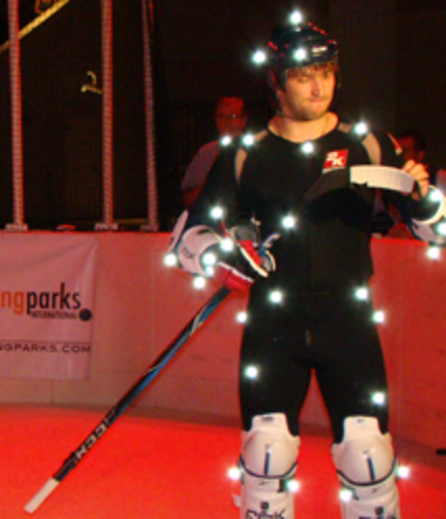
\includegraphics[height=37mm]{Chapters/2/Pics/Pdf/vicon.pdf}}
		\subfigure[]{\label{fig:mocap2}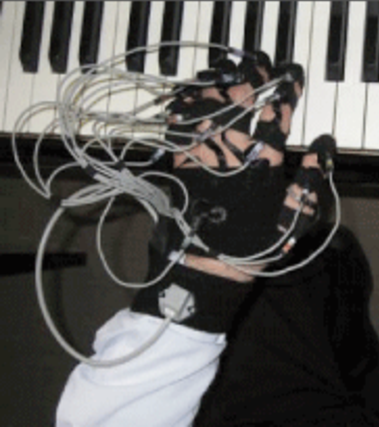
\includegraphics[height=37mm]{Chapters/2/Pics/Pdf/liberty.pdf}}
		\subfigure[]{\label{fig:mocap3}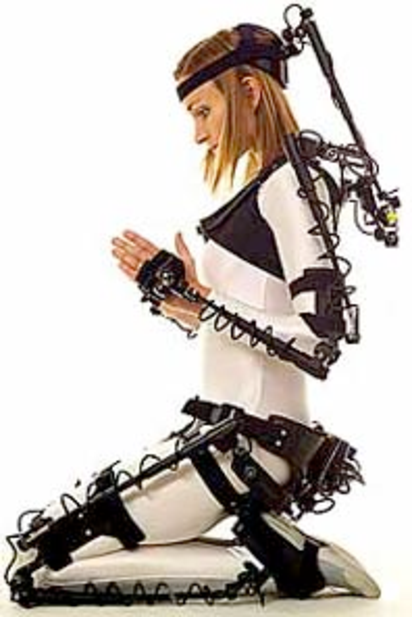
\includegraphics[height=37mm]{Chapters/2/Pics/Pdf/metamotion.pdf}}
		\subfigure[]{\label{fig:mocap4}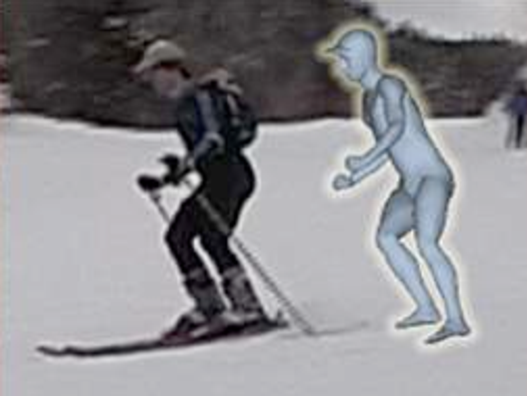
\includegraphics[height=37mm]{Chapters/2/Pics/Pdf/videomocap.pdf}}
	\end{center}
	\vspace{-0.5cm}
	\caption[Motion capture systems]{Motion capture systems, from left to right: (a) infrared camera tracking (courtesy of \citeCGA{vicon}), (b) electromagnetic tracking (courtesy of \citeCGA{polhemus, mitobe:SIGGRAPH06}), (c) electromechanical sensors (courtesy of \citeCGA{metaMotion}) and (d) video-based tracking (courtesy of \citeCGA{vlasic:TOG07}).}
	\label{fig:kinMoCap}
\end{figure}

Among intrusive methods, optical systems involve reflective markers put on real humans whose motion can be triangulated by infrared cameras, such as Vicon hardware \citeCGA{vicon}. The motion of electromagnetic sensors can also be measured relatively to a magnetic reference, such as Polhemus solutions \citeCGA{polhemus}. Another intrusive method is provided by electromechanical systems which are based on exoskeletons, such as systems provided by Meta Motion \citeCGA{metaMotion}. As shown in \myfigname \ref{fig:kinMoCap}, such hardware solutions can be quite intrusive and therefore possibly constraint the motion that is to be recorded.

On the contrary, non-intrusive methods do not rely on sensors directly in contact with captured human, and involve usually video-based processing methods, \myfigname \ref{fig:mocap4}. Such techniques appear to be a promising approach for capturing the human motion in many capture condition \citeCGA{vlasic:TOG07, qualisys}, in both indoor and outdoor environments.\\


						\noindent{\textbf{\small{Motion-driven Inverse Kinematics}}}\\

Early works among motion-driven inverse kinematics contributions aimed at infering a kinematic posture target for achieving a desired task, while preserving the characteristics (synergies, styles) of a given motion.

It has been first proposed to interpolate between available motion clips that are similar in the kinematic posture space to a posture that show the desired task \citeCGA{wiley:IEEE-TMMS97}. The cost reduction of such an approach due to the required amount of motion clips has been addressed in \citeCGA{rose:CGF01}. \citeCGA{komura:CGI03} then proposed a formulation for computing a weight matrix representing the style of a single motion example at the joint level. Such weight matrix combined with an \emph{IK} process allows to synthesize new movements while preserving the style of the original motion.

%Single motion as input: \citeCGA{tak:CGIM00} solving IK to respect end-effector targets as well as imitating an input motion. then \citeCGA{komura:CGI03} analogously provides a way of solving the IK formulation while retaining inertia and mass body features that characterize the style of a given motion as input.\\

Data reduction techniques have also been considered for representing motions in latent spaces. This generally involves the use of the Principal Component Analysis (\emph{PCA}) \citeCGA{alexa:CGF00}. It has then been shown that the respect of constraints in such PCA space combined with a prioritized \emph{IK} formulation can lead to the synthesis of new motions \citeCGA{carvalho:CAVW07}. Other solutions have been proposed for taking advantage of such latent spaces, for instance for modeling time-varying joint synergies by linear functions \citeCGA{raunhardt:VC09}.\\ % as well as motion compression in the quaternionic sapce \citeCGA{tournier:CGF09}.\\


						\noindent{\textbf{\small{Learning Methods}}}\\

The basic approach of learning methods consists in learning the mapping between kinematic configurations and end-effector tasks.

Hidden markov nodels \citeCGA{brand:SIGGRAPH00} as well as linear dynamic systems \citeCGA{li:SIGGRAPH02} have been used for learning the style of human motion examples. Models based on radial basis functions \citeCGA{rose:CGF01} and Gaussian latent variables \citeCGA{grochow:TOG04} have also been used for learning kinematic configurations with the aim of solving the inverse kinematics problem. This problem has been solved by the determination of the Jacobian inverse matrix through the learning of local transformations \citeCGA{gibet:CASA03}. The mapping between poses and style parameters can also been learnt by using Gaussian mixture models \citeCGA{wang:CAVW06}. Physical constraints can be learnt from existing motion by clustering \citeCGA{liu:TOG05}, and user-defined constraints can be taken into account by combining these latter with a statistical model learnt from motion capture data \citeCGA{chai:TOG07}. Another solution is to use Monte Carlo casting alongside with a sequential particular filtering formulation \citeCGA{courty:AMDO08}. Finally, another approach is presented in \citeCGA{aubry:GW09} to model joint synergies from existing movement sequences for solving the \emph{IK} problem.\\


%					\subsubsubsubsection{Motion Data-based Methods}
%					\label{subsubsubsubsec:CA_MC_Kinematics_Task_MoCap}

						\noindent{\textbf{\small{Motion Retrieval, Combination and Retargetting}}}\\

The ever growing availability of human motion data \citeCGA{cmumocap} has led to new research questions. Although such research directions are out of the scope of this thesis, we give some hints on research trends in extending the possibilities of motion capture databases, such as motion retrieval, motion combination and motion retargetting to cite a few.\\

Motion capture databases usually collect thousands of motion clips, creating challenges to store, access and process the data present in the database. Motion retrieval techniques usually work on two sub-problems. On the one hand it involves the identification of an adequate representation (indexing) of motion data so that high-dimension motion clips can be characterized in a low-dimension space. Secondly, reliable similarity measures have to be determined so that the comparison (retrieval) of motion chunks can be possible. %firstly finding a well-suited dimension reduction leading to a feature-based characterization of the database, secondly determining a distance metric for comparing motion chunks on this feature space.

%Early works defined dimension reduction methods such as spectral transformations \citeCGA{agrawal:FDOA93}, clustering \citeCGA{liu:CVIU03} or Principal Component Analysis (PCA) \citeCGA{forbes:SCA05}. Hand-made annotations \citeCGA{arikan:TOG03} and semantic informations \citeCGA{awad:IVA09} have also been used for reducing the dimention of motion capture databases. As for distance metrics, recent work on Dynamic Time Warping \citeCGA{kovar:SCA03} or Uniform Scaling \citeCGA{keogh:VLDB04} have yielded to reliable solutions, even if the numerical nature of the distances keep away for the moment from the desired semantic level of queries.\\

Regarding motion representations, geometric features have been proposed describing the dependencies between joints motion clips \citeCGA{muller:TOG05, lin:GRAPHITE06}. Another representation is to involve more or less automatic methods for indexing motion clips with annotations \citeCGA{arikan:TOG03, barbic:GI04, awad:IVA09}, thus characterizing differences in the semantic nature of a motion database. Other reduction methods represent motion in low-dimension spaces. Such techniques use for instance spectral transformations \citeCGA{agrawal:FDOA93}, linear reductions methods such as PCA \citeCGA{forbes:SCA05} or non-linear ones such as Isomap \citeCGA{xiang:IIHMSP07}. Clustering can also be involved in such data reduction methods \citeCGA{liu:CVIU03}.

Among simple similarity measures, works have involved measures that cope with velocity and acceleration differences, and suggest to use rotation-invariant metrics on motion clips of the same length \citeCGA{kovar:TOG02}. Another method is Dynamic Time Warping (\emph{DTW}) which gives generally good results \citeCGA{ding:VLDB08} for finding an optimal alignment between motions. Aligning two motion sequences of different time lengths in DTW has been proposed in \citeCGA{keogh:VLDB04}.\\

Highly related to motion retrieval are motion combination techniques, which aim at creating new animations from an available set of motion chunks. Multivariate interpolation has been introduced \citeCGA{rose:IEEECGA98} through a verb (motion) /adverb (interpolation) metaphor. It typically uses a verb graph linking therefore motion clips with each other, in which allowed transitions can also be computed automatically \citeCGA{kovar:SCA03}. Other techniques use motion graphs for modeling envisageable transitions between motion clips \citeCGA{kovar:TOG02}, in which annotations \citeCGA{arikan:TOG03} and path planning \citeCGA{mahmudi:I3D08} can be integrated.\\ %A linear interpolation in the PCA space has also been shown to be effective for combining new bipedal motions \citeCGA{glardon:CASA04}. 

Motion retargetting deals with the problem of adapting a given motion to other conditions or styles. Retargetting has been involved for adapting motion to different skeleton sizes \citeCGA{gleicher:SIGGRAPH98} as well as kinematic constraints \citeCGA{bruderlin:SIGGRAPH95}. Concerning style transformation, it has been observed that various frequency filtering bands can produce stylistic conditions. Emotional transformations between motion data have first been proposed in \citeCGA{amaya:GI96} based on signal processing methods. Latter works have for instance combined style translations with inverse kinematics \citeCGA{grochow:TOG04} and time warping \citeCGA{hsu:TOG05, heloir:CAVW06}.


%					\noindent{\textbf{\small{Conclusion}}}\\

%Motion data-based methods achieve a high realism in the resulting animations. However, this is mainly due to the inherent realism of captured motion. Apart from the motion-driven inverse kinematics methods detailed previously, there is for the moment no other solution in this avenue apart from capturing all possible human gestures to build an extensive motion capture database that could be used for creating any animation sequence.\\


%					\subsubsubsubsection{Task Modeling}
%					\label{subsubsubsubsec:CA_MC_Kinematics_Task_Know}

%Most of the time, motion data-based techniques still need a motion editing step which relies highly on the animator's talent depending on the desired artistic effect to accomplish. As proposed in the \emph{Biomechanics} and \emph{Neuroscience} research fields, an alternative is to consider a fine analysis of human motion, specifically by studying motion production laws that are at the origin of human motion. For a complete review of these invariant motion laws, readers are refered to \citeCGA{gibet:HdR02, hale:PhD03}.\\

%Due to the somewhat controversial statement underlying the existence of these motion laws, its use in the modeling of the motion to be animated is quite sporadic. Such invariant motion laws have nevertheless been used explicitly as motion generation laws in computer animation systems in \citeCGA{zeltzer:IEEECGA82, kopp:CA02}. Moreover, some of these motion invariants have also been invoked as quantitative criteria for evaluating the naturalness of synthesized motions \citeCGA{mataric:AAMAS99, gibet:JVLC01, kopp:CAVW04}.\\

%Many theories have been proposed to explain the mechanisms of the \emph{CNS}, a complete overview of these theories will however not be addressed in details in this bibliographic work since it would need a complete review of the Motor Control theory. Interested readers are refered to \citeCGA{hale:PhD03} for a comprehensive review. Traditionnaly, two concurrent models explain motor control tasks in Neuroscience: General Motor Programs (\emph{GMPs}) and the \emph{Equilibrium Point Control} theory. Here we will focus on \emph{GMPs} as the \emph{Equilibrium Point Control} is treated elsewhere (subsection \ref{subsubsubsubsec:CA_MC_Physics_Controllers}).\\

%\emph{GMPs} have been first introduced \citeCGA{schmidt:PR75} as a generalization of \emph{Motor Programs} \citeCGA{keel:PB68}, namely for taking into account sensory feedback that is necessary for the elaboration of spatio-temporal motor commands to produce an action. \emph{GMPs} state the existence of learning processes for assigning differently parameterized motor programs to various motion classes. This is supported by the observation of invariant laws in human motion \citeCGA{gibet:GW04}, such as:

%\begin{itemize}

%	\item the \emph{Fitt}'s law \citeCGA{woodworth:PR1899, fitts:JEP54}, which relates the movement duration to the task distance and difficulty

%	\item the \emph{isochrony} law \citeCGA{freeman:PR14}, relating the movement duration to its amplitude which was formerly observed in \citeCGA{binet:RP1893}

%	\item the \emph{two-third power} law \citeCGA{viviani:N82}, which relates the movement angular velocity to its trajectory curvature

%	\item the \emph{minimum jerk} \citeCGA{flash:N85}, stating an underlying motor command law that optimizes the smoothness of performed movements, its relation to the \emph{two-third power} law has been shown in \citeCGA{wann:JEP88}

%\end{itemize}

%Animation systems taking advantage of such human motion invariants are nevertheless quite rare, mainly because of their lack of generality since their vast majority have been demonstrated for pointing gestures. The scalability of motion invariants to other gesture types has not been demonstrated, so that elaborating control systems upon them would necessitate a fine and accurate analysis preprocess.\\


				\subsubsubsection{Conclusion}
				\label{subsubsubsec:CA_MC_Kinematics_Conclusion}

Kinematics-based animation techniques are shown to be well-suited methods when a high-level control over the task specification is needed. They give a formal framework for managing several tasks at the same time (such as secondary goals with Jacobian-based techniques) or for combining motion chunks (motion combination and retargetting).

As for inverse kinematics methods, an extensive evaluation of some of the previously cited techniques can be found in \citeCGA{unzueta:GM08}. It shows namely that neither the Jacobian transpose nor CCD formulations give satisfactory results in terms of motion quality, compared to other Jacobian-based methods.

Concerning learning techniques, one critical issue is that new motion are generally obtained by interpolating the learnt parameters, while no guaranty is provided to ensure that the resulting new movement sequences still respect the physical laws of motion.

In addition, the main drawback of methods dealing with motion retrieval and combination is that there is for the moment no other solution in this avenue apart from capturing all possible human gestures to build an extensive motion capture database that could be used for creating any animation sequence.

Despite the high realism in the resulting animations obtained by the previoulsy detailed methods, their main drawback lies in the fact that they do not deal with dynamics. Therefore, they cannot take into account the possible physical interactions of virtual characters with their environment. It is true both for simply modeling physical interactions (for instance the gravitation field or collisions) as well as reusing motion capture in different contexts (even if some hybrid methods are available, see section \ref{subsubsec:CA_MC_Hybrid}).\\

An alternative to this problem is to take advantage of the physical representation of the virtual character, so that environmental interactions can be explicitly modelled.


			\subsubsection{Physics-based Methods}
			\label{subsubsec:CA_MC_Physics}

Animation techniques based on the physical representation of virtual humans are attractive since the synthesized motion implicitly respects the physical motion laws. The virtual character is put into motion by the application of forces ($\boldsymbol{F^D}$) and torques ($\boldsymbol{\tau^D}$) so that the physical representation reaches a desired configuration $\boldsymbol{q^D}$. This scheme is called the \emph{forward dynamics} formulation, \myequname \eqref{eq:physFormulation}.

\begin{equation}
	\boldsymbol{q^D} = \mathcal{D}(\boldsymbol{F^D, \tau^D})
\label{eq:physFormulation}
\eqcaption{Forward dynamics formulation}
\end{equation}

Although there are several formulations of the motion laws (see the Lagrangian method for example \citeCGA{baraff:SIGGRAPH96, nocent:PhD01}), they are strictly equivalent to Newton's motion laws, which relate the application of forces and torques, \myequname \eqref{eq:physNewtonFormulation},  to the linear ($\boldsymbol{\Gamma}$) and angular ($\boldsymbol{\Omega}$) state of a solid characterized by a mass \emph{m} and an inertia tensor \emph{I}.

\begin{equation}
	\begin{array}{l}
		\boldsymbol{F} = m . \boldsymbol{\Gamma} \\
		\boldsymbol{\tau} = I . \boldsymbol{\dot{\Omega}} + \boldsymbol{\Omega}.I.\boldsymbol{\Omega}
	\end{array}
\label{eq:physNewtonFormulation}
\eqcaption{Newton motion laws}
\end{equation}


				\subsubsubsection{Forward Dynamics}
				\label{subsubsubsec:CA_MC_Physics_Fwd}
				
Forward dynamics implies the explicit application of time-varying forces and torques to any solid composing the physical representation $\boldsymbol{T^D}$ of the virtual character. The update of the physical configuration $\boldsymbol{q^D}$ uses an integration of solids' linear acceleration and angular velocity over time. Such a framework therefore automatically handles external influences, such as the gravitation field as well as the collisions between solids. A comprehensive study of forward dynamics basics can be found in \citeCGA{wilhelms91}.\\

The extention from the simulation of simple objects to fully articulated skeletons is far from straighforward. Early works involved the simulation of motion laws with numerical methods of high complexity. For example, the contribution from \citeCGA{wilhelms:GI85} proposed a solution with a $O(n^3)$ complexity for an articulated chain composed of \emph{n} DoFs. A recursive formulation associated to a tree structure for representing articulated bodies has then been proposed for treating such problem with a complexity reduction to $O(n)$ \citeCGA{armstrong:VC85}.\\

These early works involved the motion simulation of rigid bodies by the independent specification of forces at the joint level, which is admitted to be far too simple, since it does not take into account the integration and simulation of the internal interactions between connected bodies \citeCGA{wihelms:GI86}. Classically, an alternative is to add springed-damped effects (or equivalent) to joints for circumventing this difficulty (see section \ref{subsubsubsubsec:CA_MC_Physics_Controllers}), even if additionnal numerical instabilities then have to be counteracted \citeCGA{girard91}.\\

Despite the availability of accurate mechanical studies of human motion, such as human locomotion \citeCGA{cavagna:JP76, mcmahon:IJRR84}, these contributions generally cannot be straightfowardly integrated into simulation frameworks. Analogously to forward kinematics, the main critical issue of forward dynamics is once again to rely on the animator's intuition for finding the adequate forces and torques to put the physical model into motion.


				\subsubsubsection{Inverse Dynamics}
				\label{subsubsubsec:CA_MC_Physics_Inv}
				
An alternative is to consider the inverse of the forward dynamics formulation, the so-called \emph{inverse dynamics} (or \emph{ID}) problem. It aims at automatically computing the needed forces and torques ($\boldsymbol{F^D}$, $\boldsymbol{\tau^D}$) to be applied on rigid bodies or mechanical joints composing the physical model, so that it reaches the desired configuration $\boldsymbol{q^D}$, \myequname \eqref{eq:invPhysFormulation}.

\begin{equation}
	(\boldsymbol{F^D, \tau^D}) = \mathcal{D}^{-1}(\boldsymbol{q^D})
\label{eq:invPhysFormulation}
\eqcaption{Inverse dynamics formulation}
\end{equation}

Once the dynamic forces and torques are computed, a forward dynamics scheme is nevertheless used to put the physical model into motion. Classically, inverse dynamics methods are highly inspired from robotics, and imply either the respect of constraints along the simulation of motion laws, or the design of specific controllers. At the human body level, controllers can be considered as an \emph{internal} representation of the muscle activity that occurs between the rigid bodies composing the virtual character. Whereas constraint-based methods can be qualified as an \emph{external} formulation since they classically involve a global optimization scheme where no muscle model is provided.


				\subsubsubsubsection{Constraint-based Methods}
				\label{subsubsubsubsec:CA_MC_Physics_Constraints}

Early works have focused on the respect of geometric or kinematic constraints for finding the forces and torques to apply on articulated rigid bodies. Geometrical constraints (for example, a point belonging to an object fixed to a curve or to another object) are typically expressed linearly depending on forces and torques to be found \citeCGA{barzel:SIGGRAPH88}. It leads to the minimization of constraint equations over time. The translation and integration of these geometrical constraints into the minimization system can however conduct to an over-determined system that is difficult to solve. Another solution \citeCGA{isaacs:SIGGRAPH87, arnaldi:PhD88, dumont90} is to compute the forces and torques given a set of kinematic constraints (such as desired linear and angular displacements) that are inserted into a formulation based on the Virtual Works principle of d'Alembert. Among these early works, one of the most complete integrations of kinematics constraints into physical simulation is certainly the work presented in \citeCGA{witkin:SIGGRAPH88}. It is based on the Lagrangian formulation of physics motion laws, in which initial geometrical and physical inputs are given. It then automatically computes the required forces to respect the initial kinematic constraints, and translates the system as a minimization problem. Such an optimization problem often considers the minimization of an energy function depending on the torques $\boldsymbol{\tau^D}$.\\

Most of contributions have then focused on such optimization process, and specifically on its two main drawbacks: the control offered to users, and the computational cost of this approach. 

Concerning the first drawback, enhancing the user control has first been addressed in \citeCGA{cohen:SIGGRAPH92}, giving the possibility to the user to interact with the iterative optimizations so that the convergence to an acceptable solution can be controlled. Users can also focus on time intervals, giving a subtle control over the overall simulation. The optimization process can also be controlled if desired transitions are required \citeCGA{rose:SIGGRAPH96}. Further researchers have addressed the question of defining multi-objective functions that can cope with task priorities in the optimization process \citeCGA{abe:SCA07, jain:TOG09}.

Reducing the computational cost of such optimization-based methods has parallely been addressed, mainly by considering low-dimensional representations of virtual characters \citeCGA{popovic:SIGGRAPH00}, the motion itself \citeCGA{safonova:TOG04} or the underlying motion equations \citeCGA{barbic:TOG08}. Simplified physical constraints also make possible the preservation of dynamic effects to a reduced cost, for example through the enforcement of momentum patterns \citeCGA{liu:SIGGRAPH02}. Cost functions that can be optimized in linear time have also been under study \citeCGA{fang:TOG03} for decreasing this computational cost, highlighting a wide range of possible physical constraints such as bar and ground contact as well as flight phases.\\

Despite all these efforts, optimization-based methods are admitted to still have a high computational cost that moves away from real-time. The improvements detailed above for lowering the computational cost of such methods can also have an impact on the physical realism of the result, as attested in \citeCGA{vanWelbergen:EG09}.


				\subsubsubsubsection{Controller-based Methods}
				\label{subsubsubsubsec:CA_MC_Physics_Controllers}

Contrary to constraint-based methods, controller-based methods do explicitly model the muscle activity between the rigid bodies composing the virtual character. We can therefore consider such controllers as an integral part of the dynamic model of the virtual character. Such contributions are motivated by early works on the the Hill-type muscle model \citeCGA{zajac90}, whose spring-like effect is considered to be a key component of human postural stability:\\

" It turns out that for stable equilibrium the neuro-musculoskeletal system must possess the attributes of springs, and that for stability, these springs must exceed a certain critical stiffness. The passive, relaxed person is inherently instable at many levels. (...) Certainly the central nervous system is partly responsible for this behaviour, but the primary mode of its influence can be considered to be adjusting muscle 'spring-like' behaviour. " \citeCGA{andersson90}.\\ %p.\ 384

An explicit modeling of the Hill muscle model has been presented in \citeCGA{lee:TOG06} for a complete simulation of neck dynamics, however such an option is currently banned for real-time animation since it necessitates a highly time-consuming preprocess (neural networks) for training the controller.\\

Most of works on controller-based methods have therefore focused on simplified formulations of the Hill muscle. It has led to the design of controllers for specific motor tasks, involving for instance two types of spring-like muscle models: the Proportional-Derivative (\emph{PD}) and the Agonist-Antagonist (\emph{AA}) formulations. Researchers have also tackled the issues of automatically adapting, tuning as well as composing such controllers.\\


					\noindent{\textbf{\small{Proportional-Derivative Control}}}\\

Precursor works have studied the design and adaptation of robotics-inspired controllers to the control of virtual characters \citeCGA{raibert86, raibert:SIGGRAPH91}. In recent years, most of contributions have focused on formulating motor commands applied to each mechanical joint in terms of proportional-derivative controllers. For each joint's degree of freedom, a PD controller is attached to paired rigid bodies whose relative motion is constrained by a springed-damped effect.\\

A PD controller is therefore traditionnally composed of two terms, a proportional term parameterized by a stiffness coefficient $k_s$ and a derivative term parameterized by a damping coefficient $k_d$. The proportional term models the muscle tension effect whereas the derivative term acts as the muscle relaxation. Given the angular state of the mechanical joint ($\boldsymbol{\Theta^D}$, $\boldsymbol{\dot{\Theta^D}}$), and given a desired (target) joint configuration ($\boldsymbol{\Theta^D_t}$, $\boldsymbol{\dot{\Theta}^D_t}$), a control torque $\boldsymbol{\tau^D}$ is computed so that its application on the linked rigid bodies put them into motion towards the desired configuration, \myequname \eqref{eq:invPhysPDFormulation}.

\begin{equation}
	\boldsymbol{\tau^D} = k_s . (\boldsymbol{\Theta^D_t} - \boldsymbol{\Theta^D}) + k_d . (\boldsymbol{\dot{\Theta}^D_t} - \boldsymbol{\dot{\Theta}^D})
\label{eq:invPhysPDFormulation}
\eqcaption{\emph{PD} control formulation}
\end{equation}

A substantial amount of contributions have focused on the design of PD controllers for specific motor tasks. It includes the PD control of walking, jumping \citeCGA{hodgins:ICRA91}, stairs climbing \citeCGA{hodgins:TRA91}, as well as running, cycling, vaulting and balancing \citeCGA{hodgins:SIGGRAPH95}. PD control has also been used for simulating boxing fights \citeCGA{zordan:SCA02}, swimming motion \citeCGA{yang:SCA04}, as well as breast motion \citeCGA{zordan:SCA04, dilorenzo:TOG08}.\\

Usually, torques computed by the PD control formulation are applied with respect to the relative frame formed between the linked rigid bodies. Is has been shown however that expressing and applying the torques $\boldsymbol{\tau^D}$ towards the world frame leads to a better simulation stability \citeCGA{wrotek:SIGRAPH06}.\\


					\noindent{\textbf{\small{Agonist-Antagonist Control}}\\

Contrary to the PD controller with its unique spring model, the Agonist-Antagonist control formulation integrates two spring-like behaviors that are intended to model the spring-like behavior of two opposite agonist-antagonist muscles. \emph{AA} control is therefore composed of two tension proportional terms (parameterized by the coefficients ${k_s}_L$ and ${k_s}_H$) and a relaxation derivative term (parameterized by the damping coefficient $k_d$). Note that this formulation only needs the angular joint limits ($\boldsymbol{\Theta^D_L}$, $\boldsymbol{\Theta^D_H}$) and its current angular state ($\boldsymbol{\Theta^D}$, $\boldsymbol{\dot{\Theta^D}}$), and that no desired joint configuration is integrated into this formulation, \myequname \eqref{eq:invPhysAntagonistFormulation} \citeCGA{neff:PhD05}.

\begin{equation}
	\boldsymbol{\tau^D} = {k_s}_L . (\boldsymbol{\Theta^D_L} - \boldsymbol{\Theta^D}) + {k_s}_H . (\boldsymbol{\Theta^D_H} - \boldsymbol{\Theta^D}) - {k_d} . \boldsymbol{\dot{\Theta}^D}
\label{eq:invPhysAntagonistFormulation}
\eqcaption{\emph{AA} control formulation}
\end{equation}

In fact, this approach is based on the \emph{Equilibrium Point Control} (\emph{EPC})principle from Motor Control theory. The EPC principle argues that motor laws are not "programmed" but appear from the dynamic properties of the considered system under control \citeCGA{feldman:Biophysics66}. Human motion is then produced by transitionning between equilibrium points that are inherent to the dynamics of the human body.\\

The application of such principle is consequently equivalent to assume the existence of an equilibrium point configuration $ \boldsymbol{\Theta^D_{eq}}$ that sums all external forces $\boldsymbol{F_{ext}}$ acting on a joint to zero, according to \myequname \eqref{eq:invPhysAntagonistFormulation_EPC}:

\begin{equation}
	0 = {k_s}_L . (\boldsymbol{\Theta^D_L} - \boldsymbol{\Theta^D_{eq}}) + {k_s}_H . (\boldsymbol{\Theta^D_H} - \boldsymbol{\Theta^D_{eq}}) + \boldsymbol{F_{ext}}
\label{eq:invPhysAntagonistFormulation_EPC}
\eqcaption{\emph{AA} control formulation and Equilibrium-Point control}
\end{equation}

The motion of every joint composing the virtual character is then controlled by moving equilibrium points over time accordingly to desired configurations. This formulation has been used for example in \citeCGA{neff:SCA02} for human posture control and in \citeCGA{kry:PhD05, kry:TOG06} for grasp movement control, though with a slightly different formulation. The \emph{AA} formulation is surely the most accurate approximation of the Hill-type muscle model. It is nevertheless dedicated to the control of posture and implies ad-hoc methods for taking into account posture transitions.\\


					\noindent{\textbf{\small{Automatic Tuning and Composition}}\\

The main drawback of the controller-based approach lies in the manual process of finding adequate parameters (stiffness and damping coefficients) so that the virtual character achieves a desired motion. Due to the time-consuming trial-and-error process for determining these coefficients, and due to the proliferation of many controllers for various motor tasks, researchers have focused on the scalability of such controllers.\\

Automatic methods for determining the internal coefficients of the presented spring-like controllers have been examined. Authors suggested to use neuromotor models \citeCGA{yin:PG03} based on motion perturbations to automatically compute the coefficients. A heuristic rule has also been presented in \citeCGA{zordan:SCA02} for determining adequate coefficients according to perturbation responses. The most achieved work in such contributions is based on the expression of joint composite inertia terms \citeCGA{allen:SCA07} that leads to the automatic computation of controller coefficients for upper-body motion. These composite inertia terms are shown to be of great importance to take into account the influence of parent-child joint perturbations, which is a reason of the difficulty to find appropriate coefficients according to authors.\\

The first contribution addressing the composition of controllers has been developped in \citeCGA{vandePanne:SIGGRAPH90}. It involves the introduction of controllers whose working area can be determined in a state space. Several state-space controllers can be concatenated, where the final state of a controller is the start space of another one. Such strategy for combining controllers depending on their final-start states has been successfully applied to locomotion controllers \citeCGA{wooten:SIGGRAPH97, wooten:PhD98}. Different controllers can then be involved for controlling various phases in the same motion \citeCGA{lazlo:SIGGRAPH00, yang:SCA04}, namely by building finite-state machines. Finite-state machines have also been addressed in \citeCGA{faloutsos:SIGGRAPH01}, where the determination of pre and post-conditions defining possible transitions between controllers is automatically computed by a training/classification approach. The direct transition between controllers has also involved feedback-error learning policies for learning torque models \citeCGA{yin:TOG07}. More recently, the optimization of controllers as regards to the states of a finite-state machine has been adressed \citeCGA{wang:TOG09}, mainly by invoking biomechanical properties of human locomotion. Another recent contribution uses state exploration and reinforcement learning to synthesize task-based control schemes that are shown to be more robust than the elementary controllers they are made of \citeCGA{coros:TOG09}.


				\subsubsubsection{Conclusion}
				\label{subsubsubsec:CA_MC_Physics_Conclu}

Physics-based animation techniques show more and more compelling results for modeling the biomechanical causes that are at the origin of human motion. For instance, recent developements have shown promising results for modeling complex human systems such as a complete musculotendon model of the hand \citeCGA{sueda:TOG08}.

The main difficulty for modeling and animating virtual characters by physical models remains however to find suitable kinematic postures to feed these models. For example, in \myequname \eqref{eq:invPhysPDFormulation} and \eqref{eq:invPhysAntagonistFormulation_EPC}, a knowledge of the targetted kinematic posture is needed. This problem is in a large extent inherent to both constraint-based and controller-based methods. Generally, this issue is addressed by hybrid methods based on available motion data, in an analogous manner to kinematics methods based on motion  capture data.


			\subsubsection{Hybrid Methods}
			\label{subsubsec:CA_MC_Hybrid}

Despite many advances for giving more and more control over the chosen virtual character representation, animation techniques are still confronted to several problems. On the one hand, kinematics-based techniques struggle with the lack of interactions of the virtual character with its environment. On the other hand, physics-based methods results show quite robotic motions and still need the specification of kinematic postures.\\

Kinematics and physics-based methods therefore tend to converge towards each other, firstly by the intensive use of motion capture data. Secondly, each type of method borrows tools from its counterpart, leading to what we call here \emph{hybrid} methods.


				\subsubsubsection{Kinematics, Kinetics and Dynamics}
				\label{subsubsubsec:CA_MC_Hybrid_KinDyn}

The use of dynamic features has appeared to be a promising compromise to overcome the interaction drawbacks of kinematics-based methods. The center of mass of the virtual character has been involved in early works \citeCGA{girard:CG85} for balancing the character over its support polygon\footnote{The support polygon represents the convex hull of feet positions. A balance criterium is then proposed to ensure that the projection of the center of mass onto the ground is inside the support polygon.}. More formalized is the approach presented in \citeCGA{phillips91, phillips:SIGGRAPH91}, where the center of mass is considered as an end-effector to be controlled by an inverse kinematics approach. Works further developped in \citeCGA{boulic:EG95, boulic:CG96} improved this approach through a Jacobian-based method for controlling the center of mass (and balance) of the virtual character while respecting its mass distribution, a method which is refered to \emph{inverse kinetics}. Such an inverse kinetics scheme has also been integrated along a CCD approach \citeCGA{kulpa:Humanoids05}. Expressive balance strategies have also been addressed in \citeCGA{neff:SCA04}. The inverse kinematics scheme can also been enhanced by momentum-based features, namely for controlling a kinematic virtual character and modifying pre-captured motion under push disturbances \citeCGA{komura:CAVW05}.


				\subsubsubsection{Motion-driven Physics-based Methods}
				\label{subsubsubsec:CA_MC_Hybrid_MoCap}

Among physics-based methods that take advantage of motion capture data, constraint-based techniques have focused mainly on the modification of captured motion clips under physical motion laws. As for controller-based methods, most of works address the physics tracking of motion data.


					\subsubsubsubsection{Constraint-based Motion Modification}
					\label{subsubsubsubsec:CA_MC_Hybrid_MoCap_Modif}

Since early works in modifying motion capture data \citeCGA{gleicher:SIGGRAPH98}, there has been a substantial interest in modifying motion capture data according to physics motion laws. This has been addressed first in \citeCGA{popovic:SIGGRAPH99} by considering a simplified physical model. As stated by authors, the result is nevertheless \emph{not} physically realistic since no physics computations are processed on the full character model. Learning techniques have been therefore involved for automatically infering the physical parameters of the model \citeCGA{liu:TOG05}. The knowledge of these parameters leads to characterize the ''style'' of available motion capture data, and can produce other motions yet with the same captured style and a high computational cost. More interactive techniques then have been proposed for retiming motion capture data according to physical constraints \citeCGA{mccann:SCA06}, as well as for editing and retiming acrobatics motion under momentum-based physical laws \citeCGA{majkowska:SCA07}.

%				\subsubsubsection{Hybrid Position/Force Controller}
%				\label{subsubsubsec:CAT_Hybrid_HPF}

%\begin{equation}
%	\boldsymbol{\tau^D} = \mathcal{J}^T(\boldsymbol{q^D}) . \boldsymbol{f}
%\label{eq:invPhysHPFFormulation}
%\eqcaption{Inverse dynamics: HPF control formulation}
%\end{equation}

%$\citeCGA{paul81}, \citeCGA{craig89}, \citeCGA{sentis:IJHR05} \\ \\


					\subsubsubsubsection{Controller-based Motion Tracking}
					\label{subsubsubsubsec:CA_MC_Hybrid_MoCap_Tracking}

Early works among hybrid tracking methods involved the physics control of figures via inverse dynamics from procedurally-generated kinematic data \citeCGA{ko:IEEECGA96}. Then, the availability of motion capture data helped controller-based methods to specify the appropriate kinematic postures to be physically simulated. Most of early work among these techniques have therefore focused on tracking motion data \citeCGA{zordan:CAS99}. It includes first the design of controllers for specific motor tasks that can give responses to external disturbances, such as box punches \citeCGA{zordan:SCA02}. Such contributions mainly address the blending of kinematic postures (motion capture data) and simulated motion when needed \citeCGA{zordan:TOG05} for decreasing the computational cost of physics simulation. A more detailed organization of kinematic and dynamic controllers, as well as their transitions, has been proposed in \citeCGA{shapiro:PG03}. Motion retrieval techniques have also been investigated in such approaches so that the best suited kinematic posture can be selected, in order to drive the controllers at the right time \citeCGA{mandel:MsC04, zordan:SIGGRAPH07}.


				\subsubsubsection{Conclusion}
				\label{subsubsubsec:CA_MC_Hybrid_Conclusion}

In conclusion, the recent development of hybrid methods attests of the convergence between kinematics and physics-based methods. This convergence implies mainly an intensive use of motion capture data as well as the mixing of techniques coming from both approaches.\\

Hybrid methods based on kinematic-based techniques succeed in elaborating control schemes that can take into account physics features such as the center of mass or the momentum of virtual characters. In this type of formalisms, it is however far from straightforward to include other interactions such as ground contacts or collisions . This confirms the limitations of providing a physical realism to the kinematics-based representation of virtual characters.\\

On the other side, the combination of physics-based techniques with motion capture data makes possible the modification of pre-recorded motion clips, as well as the tracking of motion capture data with controllers. In the former case, this still induces a high computational cost that moves away from real-time. In the latter case, this does not offer an intuitive mode of control since the tracking is based on high-dimension kinematics postures (every joint positions and orientations).


		\subsection{Summary}
		\label{subsec:CA_Summary}

In this section, we have presented an overview of the modeling techniques of virtual characters, as well as the computer animation methods that are generally used for giving them life. This state of the art has reviewed kinematics-based techniques, physics-based techniques, as well as hybrid techniques taking advantage of the former two.\\

Regarding our goal to finely model the mechanisms that are at stake during percussion performances, it seems that physics-based techniques are the most adequate choice, since they offer a well-established formalism to physically control the motion of a virtual performer. Moreover, such techniques offer the opportunity to physically model the coupling between the virtual performer and a virtual instrument.

We will mainly focus on methods for motion tracking using controller-based techniques (section \ref{subsubsubsubsec:CA_MC_Hybrid_MoCap_Tracking}), since they combine our real-time requirements and the realism benefit of motion data. Two main drawbacks of such technique remain however, firstly the manual tuning of controllers' parameters, and secondly the tracking of kinematic postures of high dimension. While this thesis  will not address the first drawback, one of our contributions is to cope with the second one by using a cascaded combination of inverse kinematics and inverse dynamics controllers.

\newpage\vfill

%%%%%%%%%%%%%%%%%%%%%%%%%%%%%%%%%%%%%%%%%%%%%%%%%%%%%%%%%%%%%%%%%%%%%%%%%%%%%%%%%%%%%%%%%%%%%%%%%%%%%%%%%%%%%%%%%%%%


%%%%%%%%%%%%%%%%%%%%%%%%%%%%%%%%%%%%%%%%%%%%%%%%%%%%%%%%%%%%%%%%%%%%%%%%%%%%%%%%%%%%%%%%%%%%%%%%%%%%%%%%%%%%%%%%%%%%

	\section{Computer Music}
	\label{sec:CM}

Since its early beginnings, the main goal of \emph{Computer Music} has been to develop a novel musical medium based on computer capabilities. It involves people coming from various research areas, such as perfromers, composers, scientists and engineers. As stated below, computers offer much more possibilities compared to acoustical intruments:\\

" Man's music has always been acoustically limited by the instruments on which he plays. These are mechanisms which have physical restrictions. We have made sound and music directly from numbers, surmounting conventional limitations of instruments. Thus the musical universe is now circumscribed only by man's perceptions and creativity. " \citeCM{mathews:GV62}.\\

Two trends have then emerged from these early works, either considering computers as new instruments for synthesizing sounds, or as an help to music composition. In the first case, researchers focus on the modeling, analysis and synthesis of sound inner properties (section \ref{subsec:CM_SS}). In the latter case, it involves paradigms for controlling either natural or synthetic sounds for compositional purposes (section \ref{subsec:CM_Control}).


		\subsection{Sound Synthesis Models}
		\label{subsec:CM_SS}

Many sound synthesis models have been proposed since the advent of \emph{Computer Music}. They can mainly be divided into two sub-classes, the models that \emph{describe} sound properties (subsection \ref{subsubsec:CM_SS_Descriptive}), and those giving a physical interpretation of the \emph{source} of sound properties (subsection \ref{subsubsec:CM_SS_Physics}).


			\subsubsection{Descriptive Sound Synthesis}
			\label{subsubsec:CM_SS_Descriptive}

Among descriptive models, we will present here two of the main widespread models: \emph{sampling} and \emph{spectral} models, as a means of underlining the differences compared to physics-based models. For a more complete review about descriptive models, interested readers are refered for example to \citeCM{dePoli91, tolonen98}.


				\subsubsubsection{Sampling Models}
				\label{subsubsubsec:CM_SS_Desc_Sampling}

One of the most used synthesis models nowadays is sampling synthesis. Sampling synthesis is based on the playback of an extensive database of real pre-recorded sounds. Sampling necessitates therefore the recording of instrument sounds under a huge variety of playing conditions. This model has been used even before the advent of computer technologies, such as in the \emph{Studio de Musique Concr{\`e}te} founded in the 1950's by P. Schaeffer. Since the launch of the \emph{Fairlight CMI} \citeCM{120years}, most of current commercial synthesizers use sampling synthesis.\\

The main advantages of sampling synthesis are its straightforward implementation and its sounding fidelity since it is based on real sounds. But these advantages are however its main drawbacks. It necessitates a time-consuming process of recording sounds coming from an instrument under many playing variations. Moreover, the manipulation of sound samples requires a large amount of computer memory for storing all these pre-recorded sounds. An additional limitation is the uniqueness of the sound samples as regards to the recording conditions that prove their lack of flexibility towards environment changes.\\

Researchers have therefore developped techniques for decreasing the memory cost of such synthesis technique. This reduction can be significantly achieved by simply \emph{looping} sound samples (or just one period of it), under the assumption that the tone of the considered instrument stays constant in amplitude and pitch during the steady-state part of the sound \citeCM{roads95}.

The size of the sound sample database can also be decreased by collecting fewer sound samples than it would be needed, and process some \emph{interpolation} between these key sound samples. For example, as stated in \citeCM{smith:JNMR05}, playing back a piano sound with a given key stroke velocity can be done by interpolating "the two sounds recorded at the nearest lower and higher key velocities".

The recording of all the possible tones of an instrument can also be sidestepped by involving digital audio effects methods, so that the pitch of an original sound can be transformed to another desired pitch. This can be done by \emph{ad-hoc} methods (such as modifying the digital-to-analog clock frequency \citeCM{roads95}) or by more formalized transformations such as delay filters \citeCM{laakso:IEEESPM96}. 

More generally, the memory cost for storing the sound sample database can be reduced by applying data redution methods. This usually involves data compression techniques (such as downsampling sound samples) which may alter the quality of sound samples. Perception-based criteria can also be used for preventing the degradation of sound samples based on human perception properties \citeCM{roads95}.


				\subsubsubsection{Spectral Models}
				\label{subsubsubsec:CM_SS_Desc_Spectral}

Contrary to sampling synthesis, spectral models represent the properties of sound waves in the spectral domain. One of the most used and secular methods in spectral synthesis is the \emph{additive} model. This model considers a sound wave as the sum of sinusoidal components, just as pipe organs route air trough a selected subset of pipes. This model has been used in early electronic music, such as the \emph{Telharmonium} of Cahill \citeCM{weidenaar95}.\\ 

The additive synthesis model represents therefore the sound output $S(t)$ as the sum of the effect of oscillators characterized by time-varying amplitudes $A_i(t)$, frequencies $f_i(t)$ and phases $\phi_i(t)$, \myequname \eqref{eq:soundDescSpectralAdditive}. The oscillator characteristics define the control functions of the additive synthesis scheme. 

\begin{equation}
	S(t) = \sum_{i=0}^N{a_i(t) . \sin(2\pi . f_i(t) + \phi_i(t))}
\label{eq:soundDescSpectralAdditive}
\eqcaption{Spectral additive synthesis}
\end{equation}

These control features can be arbitrary fixed based on compositional matters, or can be obtained from the analysis of a real pre-recorded sound. Practically, the analysis stage involves a Fourier analysis, via the \emph{Short-Time Fourier} transform for instance. A peak detection is usually processed on the Fourier spectrum for obtaining the amplitudes and frequency functions. As for phase functions, most of formulations do not take them into account in the model since its importance in the additive synthesis model depends highly on the context \citeCM{roads95}. Different variations of this spectral analysis scheme have also been proposed, such as the pitch-synchronous analysis \citeCM{risset:PT69} or the phase vocoder \citeCM{flanagan:BTJ66, dolson:CMJ86}.\\

Similarly to the sampling synthesis method, the main drawback of additive synthesis is its requirement of a large number of oscillators. Data reduction methods have been proposed to decrease the number of oscillators, such as the automatic approximation of amplitude-frequency functions by line segments \citeCM{risset:PT69, strawn:CMJ80}, principal component analysis \citeCM{laughlin:MsC89}, spectral interpolation \citeCM{serra:AES90} or spectral modeling synthesis \citeCM{serra:CMJ90}.


				\subsubsubsection{Conclusion}
				\label{subsubsubsec:CM_SS_Desc_Conclusion}

Descriptive methods involve mainly either time-domain or spectral-domain techniques, coupled with signal-processing methods for taking into account various sound phenomena.\\

Compared to sampling synthesis, spectral synthesis methods are more convenient as they provide a more accurate representation of sound properties regarding human perception characteristics \citeCM{moore03}. It also provides a reduced representation cost since, firstly time-domain signals are replaced by their spectral representations, and secondly human auditory limitations can be invoked such as the human ear frequency range and simulatenous-temporal masking \citeCM{plack05}.

However, sampling and spectral models imply the use of a large amount of data (either sound samples or frequency-amplitudes functions) to finely represent sounds. It is consequently difficult to control such models for obtaining the desired sound effects when using such models.


			\subsubsection{Physics-based Sound Synthesis}
			\label{subsubsec:CM_SS_Physics}

Conversely, physical models of sound properties are generally considered to offer meaningful and intuitive control parameters over the mechanisms responsible of the sound production \citeCM{rodet94}.

The first contribution in this area has been provided in \citeCM{kelly:ICA62} for modeling human vocal strings\footnote{This first attempt turned rapidly into one of the most heard songs, since A. Clarke working with S. Kubrick on \emph{2001: a Space Odyssey} introduced the song "A bicycle built for two" composed with this model \citeCM{wood:CMJ91}}. After roughly ten years of scarcity, physical models have been explored further, either focusing on digital solutions of the wave equation governing the acoustical mecanisms occuring in various instruments, or physics models of sounding objects themselves. In this section we derive these different models for highlighting the advantages and limitations of each solution. As an illustration, we will consider in each case the classical problem of the vibrating string.


%				\subsubsubsection{Preliminaries}
%				\label{subsubsubsec:CM_SS_Physics_Prel}

%Before entering in the details of each model, we present the background inherited from early works about the problem of the vibrating string. This includes either solving a partial differential equation (\emph{PDE}) or providing a modal decomposition of the string.


%					\subsubsubsubsection{\emph{PDE}-based Solution}
%					\label{subsubsubsubsec:CM_SS_Physics_Prel_PDE}

%The vibration phenomenon of a string is classically expressed by the d'Alembert equation under adequate assumptions, \myequname \eqref{eq:soundPhysicsPDE} (see appendix \ref{sec:ssDerivation_dalembert} for a full derivation). The vertical displacement \emph{z} of the string depends on its longitudinal displacement \emph{x} over time knowing the mass density $\mu$ of the string and the applied tension $T$.

%\begin{equation}
%	\frac{\partial^2{z}}{\partial{x^2}}(x, t) - \frac{1}{c^2} . \frac{\partial^2{z}}{\partial{t^2}}(x, t) = 0\ with\ c^2 = \sqrt{\frac{T}{\mu}} 
%\label{eq:soundPhysicsPDE}
%\eqcaption{1-D d'Alembert equation}
%\end{equation}

%d'Alembert's solution to this equation is composed of two terms characterizing two travelling waves in opposite directions, \myequname \eqref{eq:soundPhysicsPDE2}. A more formalized explanation of this phenomenon is provided in appendix \ref{sec:ssDerivation_dalembertFourier} based on Fourier's solution.

%\begin{equation}
%	z(x, t) = z^{+}(ct - x) + z^{-}(ct + x) 
%\label{eq:soundPhysicsPDE2}
%\eqcaption{1-D d'Alembert travelling waves solution}
%\end{equation}

%The resulting wave of the string vibration is composed of two sinusoidal waves that propagate rigidly through the string with a velocity of $c$. The solution proposed by Fourier is more general, since it also introduces the representation of the travelling waves by a sum of \emph{normal modes} that characterize the allowed deformations of the string.


%					\subsubsubsubsection{Modal Decomposition}
%					\label{subsubsubsubsec:CM_SS_Physics_Prel_Mode}

%An alternative to the \emph{PDE}-based model is to consider the string as composed of a combination of mechanical elementary oscillators, such as masses linked by springs and dampers. A justification of the use of such model is provided in appendix \ref{sec:ssDerivation:modalDecomposition}, showing that a modal decomposition can analogously lead to the d'Alembert equation.\\

%Similarly to a \emph{PDE}-based formulation, a modal decomposition can lead to the identification of \emph{normal modes} describing the oscillations of the masses composing the system. Here we will present such a model with a simplified example composed of a coupled pair of masses. The motion of each mass is described by a second-order differential equation, \myequname \eqref{eq:soundPhysicsModalDecomposition}.

%\begin{equation}
%	\begin{array}{l}
%		m . \ddot{x_1}(t) + k.x_1(t) + k.(x_1 - x_2) = 0 \\
%		m . \ddot{x_2}(t) + k.x_2(t) + k.(x_2 - x_1) = 0
%	\end{array}
%\label{eq:soundPhysicsModalDecomposition}
%\eqcaption{1-D modal decomposition}
%\end{equation}

%By introducing the normal modes $q_1 = x_1 + x_2$ and $q_2 = x_1 - x_2$, the previous system becomes:

%$$
%\begin{array}{l}
%	\ddot{q_1}(t) + \frac{k}{m}.q_1(t) = 0 \\
%	\ddot{q_2}(t) + 3.\frac{k}{m}.q_2(t) = 0
%\end{array}
%$$

%The normal modes $q_1$, $q_2$ are uncoupled and $x_1$, $x_2$ are linearly obtained by $x_1 = \frac{q_1+q_2}{2}$ and $x_2 = \frac{q_1-q_2}{2}$. The normal deformation modes $q_1$ and $q_2$ are respectively characterized by a radian frequency equal to $\sqrt{\frac{k}{m}}$ and $\sqrt{3.\frac{k}{m}}$.


%					\subsubsubsubsection{Conlusion}
%					\label{subsubsubsubsec:CM_SS_Physics_Prel_Conlusion}

%\emph{PDE}-based and modal models are intrinsically different by nature since they provide either an \emph{analytical continuous} or a \emph{discretized} solution to the vibrating string problem. To a more general extent, researchers have focused on these continuous and discretized formulations for a wide range of instruments. In the case of the analytical formulation, it is however not always possible to provide a solution to the problem; for example the transposition of the vibrating string to a vibrating bar leads to a 4$^{th}$ order \emph{PDE} with no general solution. Continuous problems have therefore also been studied through the discretization of the wave equation governing the considered systems.


				\subsubsubsection{Digital Solution of the Wave Equation}
				\label{subsubsubsec:CM_SS_Physics_Wave}

Many methods have been proposed to provide a digital solution of the continuous formulation of the wave equation. They are usually divided into two categories, those providing a "\emph{brute-force}" solution of the wave equation, and those based on a bank of delay lines called \emph{digital waveguide}.


					\subsubsubsubsection{Preliminaries on the Wave Equation}
					\label{subsubsubsubsec:CM_SS_Physics_Wave_Preliminaries}

Before entering in the details of each model, we present the background inherited from early works about the problem of the vibrating string. This includes either solving a partial differential equation (\emph{PDE}) or providing a modal decomposition of the string.

The vibration phenomenon of a string is classically expressed by the d'Alembert equation under adequate assumptions, \myequname \eqref{eq:soundPhysicsPDE} (see appendix \ref{sec:ssDerivation_dalembert} for a full derivation). The vertical displacement \emph{z} of the string depends on its longitudinal displacement \emph{x} over time knowing the mass density $\mu$ of the string and the applied tension $T$.

\begin{equation}
	\frac{\partial^2{z}}{\partial{x^2}}(x, t) - \frac{1}{c^2} . \frac{\partial^2{z}}{\partial{t^2}}(x, t) = 0\ with\ c^2 = \sqrt{\frac{T}{\mu}} 
\label{eq:soundPhysicsPDE}
\eqcaption{1-D d'Alembert equation}
\end{equation}

d'Alembert's solution to this equation is composed of two terms characterizing two travelling waves in opposite directions, \myequname \eqref{eq:soundPhysicsPDE2}. A more formalized explanation of this phenomenon is provided in appendix \ref{sec:ssDerivation_dalembertFourier} based on Fourier's solution.

\begin{equation}
	z(x, t) = z^{+}(ct - x) + z^{-}(ct + x) 
\label{eq:soundPhysicsPDE2}
\eqcaption{1-D d'Alembert travelling waves solution}
\end{equation}

The resulting wave of the string vibration is composed of two sinusoidal waves that propagate rigidly through the string with a velocity of $c$. The solution proposed by Fourier is more general, since it also introduces the representation of the travelling waves by a sum of \emph{normal modes} that characterize the allowed deformations of the string.\\

An alternative to the PDE-based model is to consider the string as composed of a combination of mechanical elementary masses linked by springs and dampers. A justification of the use of such model is provided in appendix \ref{sec:ssDerivation:modalDecomposition}, showing that a modal decomposition can analogously lead to the d'Alembert equation.\\

PDE-based and modal models are intrinsically different by nature since they provide either an \emph{analytical continuous} or a \emph{discretized} solution to the vibrating string problem. To a more general extent, researchers have focused on these continuous and discretized formulations for a wide range of instruments. In the case of the analytical formulation, it is however not always possible to provide a solution to the problem. Continuous problems have therefore also been studied through the discretization of the wave equation governing the considered systems.

					\subsubsubsubsection{"Brute-force" Models}
					\label{subsubsubsubsec:CM_SS_Physics_Wave_FD}

Two main methods are involved in brute-force models: the finite-difference and finite-element schemes. These two formulations proceed to a discretization of the wave equation both in space and time. A good introduction to the numerical analysis of partial derivative equations can be found in \citeCM{saiac06}. Probably due to the required mathematical background, finite-element methods are most of the time eluded in the literature, so that we provide a complete derivation of these models applied to the simple vibrating string problem in appendix \ref{sec:ssDerivation:finiteDifferenceElement}.\\

The finite-difference scheme has been used since the beginning of physical models. An application to the vibrating string has been firstly proposed based on this scheme \citeCM{ruiz69, hiller:JAES71}. The finite-difference formulation has also been used for modeling the acoustic response of other musical instruments with more complex (dissipative, dispersion) phenomena, such as xylophone bars \citeCM{bork:AA95, chaigne:JASA97, doutaud:JASA98} and drum membranes \citeCM{bouenard:MsC06}.\\

The finite-element formulation has also been used in the simulation of many musical instruments, such as drum membranes \citeCM{orduna:JASA91} and bars \citeCM{bork:AAA99, bretos:AA99}. The finite-element method has also been integrated along with rigid-bodies simulation in \citeCM{obrien:SIGGRAPH01}. The \emph{Modalys} framework \citeCM{modalys} from \emph{IRCAM} \citeCM{bensoam:PhD03, ellis:ICMC05} makes also available such formulation.\\

The main advantage of the finite-difference scheme is its straighforward treatment of the discretized acoustical problem. However, its drawbacks are firstly in terms of simulation, since no control of the space-time error during the simulation is available, and secondly in terms of discretization, since such method cannot be applied to all geometries. On the contrary, from appendix \ref{sec:ssDerivation:finiteDifferenceElement}, finite-element methods provide a formal framework for controlling the error made both along space and time (based on a norm on a vectorial space), and its general discretization formulation (possibly non equally distributed) can be applied to all geometries.

However, both methods are admitted to have a high computational cost, preventing their use in real-time simulations, even if some contributions have explored a cost reduction. In the case of finite-difference, Field Programmable Gate Arrays (\emph{FPGAs}) have for instance been used for parallelizing the numerical solution of the wave equation \citeCM{motuk:ICASSP05}. %, kartadinata:NIME06}.\\


					\subsubsubsubsection{Digital Waveguide}
					\label{subsubsubsubsec:CM_SS_Physics_Wave_Waveguide}

Another alternative based on partial derivative equations is the digital waveguide formulation. Instead of discretizing the PDE that governs the acoustical response of a musical instrument, it directly proceeds to the discretization of the \emph{solution} of the considered PDE.\\

The first contribution in this area is the work from Karplus and Strong \citeCM{karplus:CMJ83}. At the beginning, this work was more an extension of the descriptive \emph{sampling} synthesis method than a physically-motivated solution. The aim was to get rid of the need of a huge amount of pre-recorded sound samples. Karplus and Strong proposed therefore an \emph{ad-hoc} wavetable scheme based on delay lines initialized by random numbers rather than real sound samples (see appendix \ref{sec:ssDerivation:dW} for the application to such a scheme to the vibration string problem).\\

A physical interpretation of the abstract solution of Karplus and Strong has then been proposed in \citeCM{smith87, smith:CMJ92}. Applied to the vibrating string problem, it involves the discretization of \myequname \eqref{eq:soundPhysicsPDE2} given a time sampling period $T_s$ and a space sampling step $X_s$ such that $X_s = c.T_s$. The discretization leads to:

$$
\begin{array}{l}
	z(x, t) \mapsto z(p.X_s, n.T_s) = z^{+}(n.c.T_s - p.X_s) + z^{-}(n.c.T_s + p.X_s) \nonumber \\
	z(x, t) \mapsto z(p.X_s, n.T_s) = z^{+}((n-p).c.T_s) + z^{-}((n+p).c.T_s) \nonumber
\end{array}
$$

\begin{equation}
	z(x, t) \mapsto z(p, n) = z^{+}(n-p) + z^{-}(n+p)
	\label{eq:soundPhysicsDW}
	\eqcaption{Digital waveguide formulation}
\end{equation}

By removing the sampling constants, the discretization leads to \myequname \eqref{eq:soundPhysicsDW}. The discretized problem of the vibrating string described by \myequname \eqref{eq:soundPhysicsDW} includes then the superposition of the effect of two nested delay lines corresponding to the two travelling waves in opposite directions, as explained in \citeCM{smith98} (see appendix \ref{sec:ssDerivation:dW}).\\

Further works on the digital waveguide approach have then explored improvements for taking into account other physical phenomena and instruments of larger (2D or 3D) dimensions. These problems are generally approached through the design of a system composed of delay lines excited by digital filters, as proposed by early works \citeCM{mcIntyre:JASA83}, in a similar way to the design of \emph{modifiers} in the work of Karplus and Strong (see appendix \ref{sec:ssDerivation:dW}). Digital waveguide methods use signal processing techniques for taking into account real physical effects. An open-source framework called the \emph{Synthesis ToolKit (STK)} is available for sharing such contributions \citeCM{stk, cook:ICMC99}.\\

Regarding physical phenomena, the accounting of loss phenomena, such as amplitude attenuation, have for example been adressed in \citeCM{valimaki:JAES96, borin:ICMC97, valimaki:JAES98}. Dispersion effects, such as frequency-dependent delays, have been presented for instance in \citeCM{rochesso:NAM96, rochesso:TSAP99}.

As stated in \citeCM{bank:PhD06}, adding such digital filters may have dramatical effects on the simulation result, so that digital control filters have to be integrated for ensuring that the result belongs to an adequate frequency range. This includes for example the introduction of simple solutions such as first-order allpass filters \citeCM{jaffe:CMJ83}, as well as more complex mechanisms such as fractional-delay filters \citeCM{laakso:IEEESPM96}.

Another difficulty arises from the complexity of nested digital filters that is the estimation of internal parameters of each digital filter included in a waveguide scheme \citeCM{smith:PhD83}. This parameter estimation generally involves the analysis of real pre-recorded instrument sounds \citeCM{karjalainen:JAES02}.\\

The one-dimensional digital waveguide approach has been used for a wide range of musical instruments \citeCM{smith:JNMR05}. For modeling instruments of higher dimensions than a string, researchers have studied the combination of one-dimensional digital waveguides. This includes the introduction of 2D \citeCM{vanDuyne:ICMC93} and 3D \citeCM{vanDuyne:ICMC96} waveguide meshes.

Digital waveguide models have also involved the modeling of the instrument bodies. It includes either post-processing digital filters for rendering the reverberation of sounds in body cavities \citeCM{garnett:ICMC87} or commuted synthesis techniques \citeCM{karjalainen:SMAC93}.


%					\subsubsubsubsection{Conclusion}
%					\label{subsubsubsubsec:CM_SS_Physics_Wave_Conclusion}

%Finite-difference and finite-element methods proceed to the discretization of the \emph{PDE} governing the acoustical system under study, whereas digital waveguide focus on the discretization of the \emph{solution} of such \emph{PDE}. As stated previously, the main drawback of finite-difference and finite-element techniques is their computational cost that moves away from real-time sound synthesis.

%On the contrary, digital waveguides are less cost-expensive, mainly because they provide directly a discretization of the \emph{PDE} solution. The critical issue in this type of method is however the assumption that such a solution exists. This is not always the case, so that digital waveguide methods tend to provide additional digital filters for taking into account physical phenomena, leading to an approximated solution to the acoustical problem that is considered. Such approximations reveal also the difficulty of waveguide approaches to take into account non-linearities.


				\subsubsubsection{Modal and Mass-Spring Models}
				\label{subsubsubsec:CM_SS_Physics_SO}

The main difference between modal or mass-spring models compared to the models based on the wave equation detailed in the previous section is the implicit or explicit spatial discretization of the acoustical object under study. To that mean, the models based on the wave equation proceed to an implicit spatial discretization since this discretization is invoked for discretizing the PDE both in space and time. 

Conversely, modal and spring-mass models do not make any assumption of the PDE governing the acoustical system, and directly discretize the sounding object spatially, and then also in time for solving the mechanical problem. These two methods differ from the elementary objects they involve in their formulation, either 2$^{nd}$ order oscillators or masses connected with springs.

%We discuss in this section the theory underlying the modal synthesis method, and more generally the techniques involving a mechanical decomposition of the sounding objects. It should be noted we consider here the modal synthesis as a mechanical formulation composed of mechanical elements (masses, springs, dampers). In fact modal synthesis can also be interpreted as a source-filter method composed of a bank of second-order resonators (or filters). For details concerning this last interpretation readers are refered to \citeCM{adrien:PhD89, avanzini09}.\\


					\subsubsubsubsection{Modal Synthesis}
					\label{subsubsubsubsec:CM_SS_Physics_SO_ModalSynthesis}

The modal formulation expresses the discretization of an acoustical system as a bank of 2$^{nd}$ order oscillators, each representing a mode of vibration of the sounding object. The modal formulation has been first introduced to sound synthesis in \citeCM{adrien:PhD89, adrien91}, these works are typically the fundamental basis of the \emph{Modalys} framework \citeCM{modalys}. In this paragraph we will focus on a system represented by a network of $N$ undamped oscillators, which can be characterized by a matricial equation \myequname \eqref{eq:soundPhysicsMM} containing the governing equation of each ocillator.

\begin{equation}
	\boldsymbol{M} . \ddot{\boldsymbol{z}}(t) + \boldsymbol{K} . \boldsymbol{z}(t) = 0
	\label{eq:soundPhysicsMM}
	\eqcaption{Modal synthesis formulation}
\end{equation}

The matrices $\boldsymbol{M}$ and $\boldsymbol{K}$ are referred to the mass and stiffness matrices. These are usually not diagonal, so that the system is characterized by $N$ coupled oscillators. By introducing the notion of \emph{modal shapes} $\boldsymbol{S}$ (see appendix \ref{sec:ssDerivation:mM}), this system can be rewritten in the form of a system of $N$ \emph{uncoupled} oscillators representing the normal vibration modes $\boldsymbol{q}$ of the system. $\boldsymbol{q}$ represents then an orthogonal basis of the system, such that $\boldsymbol{z}$ can be expressed as a linear composition of $\boldsymbol{q}$, \myequname \eqref{eq:soundPhysicsMM2}.

\begin{equation}
	\forall j \in [1, N]\ z_j(t) = \sum_{i = 0}^{N} s_{i, j} . q_i(t)\ \Leftrightarrow \ \boldsymbol{z} = \boldsymbol{S} . \boldsymbol{q}
	\label{eq:soundPhysicsMM2}
	\eqcaption{Modal synthesis formulation, linear combination of normal modes}
\end{equation}

The interest of the modal formulation is that it does not make any assumption on the considered system. Such a formulation can moreover be shown to be equivalent to a continuous representation based on PDE. This affirmation is justified in appendix \ref{sec:ssDerivation:mM}. The modal method has inspired many works since its introduction to sound synthesis, mainly because one of the most important advantages of such a formulation is its compatibility with an analysis stage. This last one may be used to determine the adequate basis (\emph{normal modes}) necessary for describing a particular acoustical system. Analytical techniques have been developped for determining such features depending of the shapes of sounding objects \citeCM{vanDenDoel:ICAD96, vanDenDoel:Presence98}. These can also be obtained from measurements on real objects \citeCM{pai:SIGGRAPH01, corbett:Presence07}.


					\subsubsubsubsection{Mass-Spring Networks}
					\label{subsubsubsubsec:CM_SS_Physics_SO_MSN}

An equivalent approach, the CORDIS-ANIMA framework \citeCM{cadoz:PhD79, luciani:PhD85, razafindrakoto:PhD86, cordis}, is based on an analogous mechanical formulation, modeling any musical instrument as a network of mass-spring elements \citeCM{florens91, cadoz:CMJ93}. This system has the advantage to treat the evolution of any sounding object at the sound sampling frequency (about $44\ kHz$). Such method is generally admitted to have a critical performance cost, although real-time simulation can be reached and combined to specific hardwares in particular cases \citeCM{luciani:ENACTIVE07}. CORDIS-ANIMA has particularly been the basis in a musical composition perspective, for example through the introduction of Genesis$^3$ \citeCM{castagne:JIM09}. %However, as attested by the authors \citeCM{castagne:JIM09}, it generally cannot be used for real-time sound synthesis although some efforts have been made to propose specific hardwares to reach real-time in particular cases \citeCM{luciani:ENACTIVE07}.


				\subsubsubsection{Conclusion}
				\label{subsubsubsec:CM_SS_Conclusion}

Physics-based methods focus either on the PDEs (or their solutions) governing the considered acoustical system, or on physics-based alternative which consist in providing a discretization of sounding objects into elementary structures (oscillators or mass-spring systems).\\

Hybrid methods have also been explored for combining the assets of both PDE-based methods with modal or mass-spring representations. Some works have for instance mixed a finite-element method to a modal synthesis formulation \citeCM{obrien:SCA02}, or a combination of modal and mass-spring representations \citeCM{raghuvanshi:I3D06} for generating sounds from rigid-body simulations. Acoustical features such as radiation factors \citeCM{james:TOG06} as well as frequency-masking can also be used \citeCM{vanDenDoel:Presence04} for enhancing the sound realism in virtual scenes.\\

The choice of a physics-based method is characterized by a compromise between real-time requirements and the techniques involved in the models. Finite-difference and finite-element methods typically fall short in real-time difficulties. Digital waveguides are quite low cost-expensive. However it generally involves the introduction of \emph{ad-hoc} filters for taking into account physical phenemona that cannot be solved by a general PDE. The modal formulation expresses any musical instrument (and more generally any sounding object) as a finite network of oscillators. This method is admitted to be powerful for the main reason that no underlying assumption is made in such a model, compared to physical models based on PDEs. Such a formulation is characterized by a high computational cost, however in practice the normal modes are usually precomputed so that the physical sound synthesis can run in real-time. Other speed-up improvements have also been proposed based on mode compression and truncation \citeCM{vanDenDoel:Presence04, raghuvanshi:I3D06}, as well as spectral representations \citeCM{bonneel:TOG08}.


		\subsection{Gestural Control of Sound Synthesis Processes}
		\label{subsec:CM_Control}

Another research area in \emph{Computer Music} is to explore how the previously detailed sound synthesis techniques can be involved in a musical composition process. This research direction addresses the \emph{control} of sound synthesis processes. Such a question has been present since the beginnings of \emph{Computer Music}:\\

" Today, scientists and musicians (...) are trying to make the computer play and sing more surprisingly and mellifluously. As a musical instrument, the computer has unlimited potentiallities for uttering sounds. (...) Wonderful things would come out of that box if only we knew how to evoke them. " \citeCM{pierce:Playboy65}\\

%In this development, we present the three major trends in the control of sound processes. A first research direction concerns the composition of performances for computers as well as the live interaction with sound processes (subsection \ref{subsubsec:CM_Control_AC}). Another direction deals with providing tools so that performers can interact with machines, leading to interactive performances (subsection \ref{subsubsec:CM_Control_IP}). Lastly, the control of sound synthesis paradigms can be achieved by the availability or the modeling of instrumental gesture mechanisms (subsection \ref{subsubsec:CM_Control_GC}).

It attests the fact that research works have provided many sound synthesis formalisms competing more and more in accuracy, but also forgot on this way the corporal (gestural) strategies that are involved to give them birth in instrumental performances. The last decades have therefore focused on solutions for proposing paradigms in order to recover this corporality. Such research direction is generally addressed as a means of \emph{controlling} sound processes, either by involving the design of devices for capturing instrumental gestures, or by proposing models of these latter.

In this development, it should be noted that we will refer to \emph{gestures} as the actions that can be performed by a user. We will not address a complete bibliographic review of gesture typologies for characterizing the differences between effective, accompanying or figurative gestures in the case of a music performance. Interested readers looking for an extensive review on these typologies are referred to \citeCM{gibet:PhD87, cadoz94, wanderley:PhD01, jensenius:PhD07}. %\citeIPA{gibet:PhD87} 


%			\subsubsection{Automatic Composition and Interactive Performances}
%			\label{subsubsec:CM_Control_AC}
%			
%One of the first tentative of an automated musical composition by computers dates back to the 1950s with the "Illiac suite" \citeCM{hiller59}. These experiments have largely proved that standard musical composition techniques could be handled by computer programming, with a huge controversy about the replacement of humans by computers.
%
%Nowadays, such a controversy does not hold anymore, mostly due to the popular and every-day use of electronic technologies. Some contributions have also made their own speciality to create music peformances from computers, as attested by the creation and proliferation of electronic music orchestras, or \emph{laptop orchestras} \citeCM{plork, slork}.\\
%
%Due to the quite recent emergence of automatic composition, there are as many terms for naming it\footnote{Depending on authors and terminologies, automatic composition is also called algorithmic composition, computer composing, score synthesis, machine musicianship. For details on these terminologies, see for example \citeCM{miranda00} (pp. 9--10)} as the number of techniques involved in the related contributions. We will mainly focus on techniques for organizing sound synthesis processes including explicit rules, stochastic, learning and evolutionnary systems.
%
%Systems based on explicit rules are the simplest form of automatic composition. Such rules are typically hard-coded in the system, and can take into account a set of transformations on pre-recorded sounds or specific styles of composition \citeCM{todd91}. For example, these rules can be derived from composer style, as achieved in \citeCM{shottstaedt89} for mimicrying the counterpoint compositional style of Palestrina.
%
%Not surprisingly, rule-based techniques lead to well-defined results, but leave most of the time little room to expressiveness and improvisation. Stochastic models can be an alternative to that mean, based on randomness and probabilistic models. One of the most well-known works in this area is the one of Xenakis \citeCM{xenakis01}. More recently, a stochastic approach has been used for modeling the breakbeat style of Squarepusher \citeCM{collins:ARIADA03}.
%
%Statistical techniques have also been combined with learning techniques to take into account a predetermined rythmic and phrasing style. The extraction of statistical features of targetted inputs have been explored by using Markov models and artificial neural networks \citeCM{tovainen:MP95}. Learning techniques are commonly used as non-linear statistical data modeling techniques, for example for finding patterns in musical data. Such formulations are most of the time quite effective, but as stated in \citeCM{mozer:CS94}, what is statistically relevant is unfortunately not always pertinent to a musical ear, so that it is in general difficult to predict what structure will be learned in such approach.
%
%Evolutionnary approaches model the Darwinian conception of evolution by random variation and natural selection of a population. Genetic algorithms have been extensively explored in automatic composition \citeCM{bentley01}. A genetic approach can be used both for modeling low-level problems, such as modeling the evolution of amplitude/frequency modulation patterns \citeCM{dahlstedt:Leonardo01}, and high-level models such as the evolution of bird songs \citeCM{werner:ECAL97} or a cultural approach of the evolution of sound repertoires among a population \citeCM{miranda:CMJ02}.\\
%
%Conversely, the research field of interactive performances does not address the composition of performances for machines, but interaction paradigms for giving the possibility to performers to interact with sound processes during live performances. These methods are usually admitted to distinguish two main strategies, based either on \emph{score-following} or \emph{performan-ce-oriented} techniques.
%
%\emph{Score-following} strategies initiated in \citeCM{dannenberg:ICMC84, vercoe:ICMC84} aim at proposing interaction mechanisms during live performances so that computers can react to performers' actions. These techniques most of the time involve stochastic approaches for recognizing and reacting to pitch and tempo changes during music performances. This feature detection can for instance include Markov models combined with stochastic observations of audio and tempo \citeCM{raphael:PAMI99, orio:ICMC01, raphael:ML06}.
%
%Conversely, \emph{performance-oriented} systems is described in \citeCM{rowe93, rowe01}. Such an approach offers the possibility to performers to interact with machines while preserving their musical style. This also allows the setup of a discussion or improvisation where machines not only react but also learn and propose adequate musical themes to performers in live performances \citeCM{zicarelli:CMJ87, pachet:IEEEMultimedia02, assayag06}.
%
%The use of interfaces has also been explored by other contributions for specifying the interaction between sound synthesis processes during live performances \citeCM{zadel:NIME06, zadel:ICMC08}.
%
%
%				\subsubsubsection{Conclusion}
%				\label{subsubsubsec:CM_Control_AC_Conclusion}
%
%Automatic composition methods more generally borow tools from the artificial intelligence research area. One of the most critical issues in these works is the discussion of the quality of the automated compositions by computers. As stated in \citeCM{miranda:GECC00}, the question of whether or not computers can compose music is not relevant anymore, but an open question is how to evaluate these compositions: "We are often unable to judge these computer-generated pieces because they tend to lack those cultural references that we normally hold on to when appreciating music". This evaluation problem may also arise from the fact that no sensory feedback (apart from sound) is available for evaluating the compositions generated by computers.\\


%			\subsubsection{Gestural Control of Sound Synthesis}
%			\label{subsubsec:CM_Control_GC}

%Another research direction aims at studying the influence of instrumental gestures on the control of sound processes. This traditionally involve two main streams, either works providing devices (or \emph{gestural controllers}) that composers and instrumentists may use for controlling sound synthesis processes, or contributions analysing and modeling instrumental gestures with an emphasis on their influence on musical playing codes and their resulting sounds.
%Another research direction aims at providing devices that composers and instrumentists may use for controlling sound synthesis processes. These devices are generally called \emph{gestural controllers} as they are based on sensor technologies for capturing specific features contained in instrumental gestures.\\

%The great interest about instrumental gestures has also emerged, mainly with underlying goals of analysing and modeling the influences of gestures on musical playing codes and their resulting sounds.\\


			\subsubsection{Acquisition, Mapping and Digital Instruments}
			\label{subsubsubsec:CM_Control_GC_GA}

Capturing gesture characteristics are an important part of the design of devices for controlling sound synthesis processes. These devices are generally refered as digital music instruments (\emph{DMIs}), including the design of a controller capable of acquiring and making a correspondance between gesture characteristics and sound synthesis processes. The nature of these characteristics will therefore influence the choice of sensor technology that will be incorporated to the device.\\

Once the input device is built and embeds the chosen sensor technologies, another issue arises then for specifying how the numerical conversion of the identified gestural characteristics should act on the inputs of a sound synthesis process. This issue is commonly known as the \emph{mapping} problem.


					\subsubsubsection{Direct and Indirect Acquisition}
					\label{subsubsubsec:CM_Control_GC_GA_D}

There are basically two ways of capturing gestural characteristics for the design of DMIs, either direct or indirect solutions.

Direct acquisition methods make use of sensors for monitoring the actions performed by users on the device. These sensors can be of different nature and capabilities for capturing various features. An extensive review on the use of these sensors applied to music performances is available in \citeCM{miranda:AR06, malloch:MsC07}. These sensors can acquire both the external (action on the device) and internal (performer state) activities of the performer. To cite a few, external sensors can be magnetic or optical systems \citeCGA{vicon, polhemus} for capturing the motion of performer's body parts, or less intrusive mechanisms that can be embedded to the device such as force-sensitive resistors, potentiometers or tactile-position sensors. Sensors can be use to measure the internal activity of the performer as biosignals, namely by capturing electromyogram (\emph{EMG}) data. EMG data have been used for example for capturing conducting gestures \citeCM{marrinNakra:PhD00}.

On the other hand, indirect acquisition methods proceed to the identification and extraction of gesture characterisics from sounds of acoustic instruments. Signal processing techniques are generally the basis of these methods for extracting sound features that charaterize gesture features such as the position of the device, the performed fingering or the strike location on a drum membrane \citeCM{wanderley:IEEE04}. Such techniques have among other instruments been applied to the acoustic guitar \citeCM{traube:NIME03} and clarinet \citeCM{egozy:MsC95}.


					\subsubsubsection{Mapping}
					\label{subsubsubsec:CM_Control_GC_GA_M}

Mapping can be defined as the gesture-sound relationship, that is how numerical data acquired from sensors are related to the inputs of sound synthesis processes. Although a mapping with basic one-to-one relations between gesture outputs and sound inputs should be the most straightforward and evident solution, it is now admitted that complex mappings are more suited since acoustical instruments are characterized with a non-linear and complex scheme for relating gesture and sound \citeCM{hunt:ICMC00}.

Two main strategies have been therefore proposed for solving this mapping issue. The first solution is to explicitly express the mapping rules based on \emph{a priori} knowledge on acoustical systems \citeCM{hunt00, vanNort:NIME04}. Another alternative is to automatically generate the gesture-sound mapping, for example by training artificial neural networks \citeCM{cont:NIME04} or processing a data reduction for keeping the most statistically meaningful features \citeCM{bevilacqua:SIMS02}. Generative methods for achieving the mapping is however quite arbitrary since such learning or statistical techniques do not ensure that the resulting statistical discrimination corresponds to gestural differences.

The mapping between gestural data and sound synthesis processes is therefore of paramount importance when designing a DMI, it may influence in particular the way performers can interact with the device. The design of the mapping can also be seen as an attribute of the composition process, since the way the mapping is expressed can influence the use of the gestural controller \citeCM{doornbusch:OS02}.


				\subsubsubsection{Digital Music Intruments}
				\label{subsubsubsec:CM_Control_GC_DMIs}

The design of DMIs has been explored much before the advent of \emph{Computer Music}, by building electric and/or electronic interfaces for generating sound from novel control surfaces that could be used by performers. One of the most well-known early achievements in this domain is the Theremin invented in the 1920s by Lev Termen \citeCM{theremin}. With both the growing availability and democratization of personal computers and the widespread use of the MIDI protocol \citeCM{midi}, research works dealing with the design of DMIs have increased drastically \citeCM{chadabe97}. %Similarly to the apperance of automatic composition (laptop) orchestras, digital music orchestras have also been formed for exploring the performance possibilities of \emph{DMIs} \citeCM{pestova:ICMC09}.\\
It has especially led to the appearance of digital music orchestras for exploring the performance possibilities of DMIs \citeCM{pestova:ICMC09}.\\

An extensive classification of DMIs is available in \citeCM{miranda:AR06} according to their relationship to existing traditional acoustical/electric instruments. In this development we focus specifically both on \emph{augmented} and \emph{alternate} controllers.

DMIs based on augmented instruments extend existing instruments by adding sensors such as the sensors discussed in subsection \ref{subsubsubsec:CM_Control_GC_GA_D}. They provide extra control parameters to performers to those traditionaly available with existing instruments. Augmentation solutions have been explored for a wide range of musical instruments. Augmented flutes have been elaborated for mapping the breath stream \citeCM{daSilva:NIME05} and the position/orientation of the device \citeCM{palacio:NIME08} to sound synthesis processes. This principle has also been applied to electric guitars, by including for example a touchpad to a bass guitar \citeCM{bahn:NIME01} or contact sensors for enhancing an electric guitar with percussive playing techniques \citeCM{lahdeoja:NIME09}.

Conversely, alternate gestural controllers do not specifically refer to an existing traditional instrument, but rather elaborate novel musical interfaces from scratch or directly based on other objects. Such interfaces are usually based on hardware for sensing the actions of performers on the DMI. Many solutions have been proposed for capturing these actions, such as computer-vision methods \citeCM{jorda:ICMC05}, pressure \citeCM{thunder} or capacitive sensors \citeCM{malloch:NIME07}, as well as tablet devices \citeCM{zadel:NIME06, dalessandro:NIME07, zadel:ICMC08}. Other alternate controllers also integrate haptic feedback so that performers can perceive the result of their actions on the devices. This ranges from simple vibro-tactile feedback \citeCM{rovan00} to the simulation of the "feel" of the device from haptic devices \citeCM{cadoz:CMJ90, sinclair:IC08}.


			\subsubsection{Gesture Analysis and Modeling}
			\label{subsubsec:CM_Control_GC_GAM}

Conversely to works detailed in the previous section, research works have been trying not only to capture instrumental gestures, but also analyse and propose models of gesture mechanisms that can take into account all their subtle variations as regards to musical variations.\\

This includes the study of the influence of dynamics and tempo on bow gestures \citeIPA{rasamimanana:GW05, rasamimanana:GW07}. Other works have also studied anticipation phenomena that occur in instrumental gestures under musical nuances and tempo changes, this has been done for instance for bow \citeIPA{rasamimanana:JNMR08}, percussion \citeIPA{dahl:JNMR00, dahl:AAA04} and piano \citeIPA{loehr:EBR07} gestures. Mechanisms showing the influence of instrumental gestures on the audio-visual perception of instrumental performances have also put in evidence \citeIPA{wanderley:JNMR05, dahl:MC07}.\\

%influence of gestures on sound (demoucron, schooderwaldt)\\
%analysis: clustering, classification VS. hmm VS.\\

Most of models of instrumental gestures propose parameters that can take into account the direct interaction with sound processes. Such works differ mainly from their positioning towards the sound model. Some are proposing models for exciting directly the parameters of sound synthesis schemes, whereas some propose more high-level models by offering methods for generating these parameters.

Models dealing with the direct excitation of sound synthesis parameters have been proposed for instance for controlling bowed strings \citeIPA{demoucron:PhD08} by the specification of attack parameters, or for drum models \citeIPA{avanzini:PhD01, avanzini:SMC04} by the proposition of various contact models. As for higher-level models, some works have proposed the use of existing motion data. This can take the form of the optimization of a dynamic system by the addition of effort costs \citeIPA{rasamimanana:JNMR08}. Another solution is to propose a system able to "follow" and recognize motion data by the training of an hidden markov model \citeIPA{bevilacqua:NIME07, bevilacqua:GW09}. Finally, other contributions have proposed physical models for the whole gesture-sound system \citeIPA{gibet:PhD87}. In this work, the playing of a musical instrument can be conceived through the coupling of two physical models, the sound-producing gesture and the instrument. The entire gesture model can be identified using a slowly evolving mechanical model with force feedback. This has led to the proposition of a composition system through an analysis/synthesis approach \citeIPA{gibet:ICMC88}.


			\subsubsection{Conclusion}
			\label{subsubsec:CM_Control_Conclusion}

We have examined the two main streams of research works for controlling sound synthesis processes.

On the one hand, the control of sound synthesis processes can be achieved by the design of gestural controllers, involving gesture acquisition methods and exploring mapping schemes for relating the captured gesure characteristics to sound synthesis inputs. The most critical issue in this approach is the mapping between the extracted gestural data and the sound synthesis inputs.\\

On the other hand, research works in the control of sound synthesis have involved the direct modeling of gestures, by extending the current knowledge on instrumental gestures of various types, as well as providing models of interaction gestures that are strongly related to sound synthesis parameters.


		\subsection{Summary}
		\label{subsec:CM_summary}

We have drawn in this section an overview both concerning the main sound synthesis models and the strategies for controlling sound synthesis processes. The sound synthesis models involve either descriptive methods for modeling the observation of sound properties, whereas physics-based techniques model the physics phenomena at the origin of these sound properties. We have also reviewed control paradigms of sound synthesis processes that include either the design of digital music instruments or models of instrumental gestures.\\

Regarding our goal to finely model the interaction between a virtual percussionist and sound synthesis processes, it seems that physics-based sound synthesis models are an adequate solution. Specifically, the modal formulation appears as the best choice for our real-time and complexity requirements. Concerning the mapping problem, another reason in favor of physics-based sound synthesis models is the possible explicit mapping based on the physics events that are available from the simulation of the virtual percussionist and the physics parameters of the chosen sound synthesis scheme. It should however be noted that the major difference between such a mapping and the one discussed previously lies in the fact that virtual gesture characteristics will be here extracted from the simulation of the virtual percussionist, compared to a mapping using gesture characteristics coming from natural gestures. This thesis will thus present a solution of the mapping problem in the particular case of the synthesis of virtual performances.\\

Furthermore, our work comes under the category of the analysis and modeling of instrumental gestures rather than in the design of control devices of sound processes. Our major contribution is to propose a model whose design is guided by a preliminar analysis of real mechanisms occuring in percussion performances. Our model is also able to synthesize whole movements, including preparation, interaction and retraction gestures, compared to related works focusing only on interaction gestures.

%physics-based sound synthese for two reasons:
%* meaningful parameters of the acoustical problem, that can achieve real-time
%* mapping, explicit beacause physics since generative mapping based on stat or PCA do not ensure that the statistical discrminiation will be heard

\newpage\vfill


%%%%%%%%%%%%%%%%%%%%%%%%%%%%%%%%%%%%%%%%%%%%%%%%%%%%%%%%%%%%%%%%%%%%%%%%%%%%%%%%%%%%%%%%%%%%%%%%%%%%%%%%%%%%%%%%%%%%


%%%%%%%%%%%%%%%%%%%%%%%%%%%%%%%%%%%%%%%%%%%%%%%%%%%%%%%%%%%%%%%%%%%%%%%%%%%%%%%%%%%%%%%%%%%%%%%%%%%%%%%%%%%%%%%%%%%%

	\section{Virtual Music Performances}
	\label{sec:SMP}

In this section, we finally examine the contributions of both \emph{Computer Animation} and \emph{Computer Music} research fields to the synthesis of virtual music performances. We define "virtual music performances" as the \emph{modeling} of all protagonists acting during a \emph{real} music performance, \emph{i.e.} modeling techniques for representing the performer, the instrument and the interaction between the two.


		\subsection{Computer Animation Contributions}
		\label{subsec:SMP_CAC}

Early works have explored the synthesis of virtual scenes including sounding objects with a motion-driven methodology \citeCGA{takala:SIGGRAPH92, hahn:JVCA95}. These contributions however do not model a music performer explicitly, but rather consider virtual objects whose kinematic motion influences the sound rendering. Similar works have explored motion-driven methods for modifying pre-recorded sound clips \citeCGA{cardle:SCA03} or physics-based animation techniques for animating sounding rigid bodies \citeCGA{obrien:SIGGRAPH01, obrien:SCA02}.\\

Other contributions aim at animating virtual models from sound representations. The most explored solution includes works for animating virtual models from MIDI scores \citeCGA{lytle:SIGGRAPH90, lytle:SIGGRAPH01, animusic}. Such a strategy has also been proposed along with an explicit model of a kinematic representation of a virtual performer \citeCGA{woodGaines:MsC97}. Other works have proposed eiher the animation of kinematic virtual models directly from sound clips \citeCGA{cardle:SIGGRAPH02}, or the animation of a kinematic hand model from guitar tablatures \citeCGA{elkoura:SCA03}.\\

Most of the time, the contributions from the \emph{Computer Animation} research area elude both the questions of the fidelity of the synthesized motion and the interaction between virtual models with sound synthesis processes. Specifically, the relationship between virtual objects (or virtual performer models) and real instrumental gestures is generally not addressed, so that there is no way to say whether or not the synthesized gestures are similar to real-world mechanisms.

Similarly, apart from the case of MIDI-controlled animated models, the interaction between virtual models with sound processes is rarely explicited. It should moreover be noticed that animated models from MIDI scores consider the inverse mechanism of real instrumental performances. They indeed animate virtual models from the event-based struture of MIDI scores, whereas real instrumental performances show obviously that sounds result from the performer actions on sounding objects.

\newpage\vfill


		\subsection{Computer Music Contributions}
		\label{subsec:SMP_CMC}

The \emph{Computer Music} community has been prolific for providing models that can be used in virtual music performances. and especially for virtual percussion performances. It includes either percussion sound synthesis models, percussion gestural controllers and virtual percussion systems.


			\subsubsection{Percussion Sound Synthesis}
			\label{subsec:SMP_CMC_SS}

Most of sound synthesis models have been explored and applied to the specific case of percussion performances. These include finite-difference schemes \citeCM{bouenard:MsC06} accelerated with Field Programmable Gate Arrays (\emph{FPGA}) \citeCM{bilbao:DAFX05, bilbao:ICMC05} and the specification of a meaningful and explicit mapping strategies \citeCM{chuchacz:NIME07}. 2D and 3D waveguides meshes have also been applied to percussion sounds \citeCM{fontana95, aird:ICMC00}.\\

More related to virtual performances is the contribution presented in \citeCM{avanzini:ICMC01, avanzini:SMC04, avanzini:CAVW06} since these works have been combined to offer a virtual multimodal application concerned with the simulation of contact sounds. It nevertheless does not include a model of a virtual performer, but rather relies on haptic devices for exciting contact sound models with a 3D visualization feedback.


			\subsubsection{Percussion Gestural Controllers}
			\label{subsec:SMP_CMC_PC}

Several gestural controllers applied to percussion have been developed, such as the Lightning and Thunder controllers \citeCM{lightning, thunder}, the Radio Baton \citeCM{boie:ICMC89} and the Korg Wavedrum \citeCM{rule:Keyboard95}. An extensive historical review of such early works is available in \citeCM{aimi:PhD06}.\\

Percussion controllers have been extensively used for controlling sound synthesis processes. This includes signal processing techniques combined with augmented instruments for enhancing European \citeCM{aimi:MsC02, marshall:NIME02, aimi:PhD06} or Indian \citeCM{kapur:JNMR03, kapur:NIME04, kapur:PhD07} percussion instruments. A complementary approach to the growing number of gestural percussion instruments is to evaluate such devices towards the accuracy and the naturalness qualities they offer in a performance situation \citeCM{collicutt:NIME09}.\\

Despite the quality and variety of such percussion controllers, these works are not directly related to virtual performances since they are mainly used for reacting to natural gestures performed by users. To our knowledge, the only work that can be related to virtual performances is the one developped by A. Kapur on Indian percussion instruments as we will see in the next section.

%\newpage\vfill

%\citeCM{marshall:ICMC02}, \citeCM{kapur:NIME02}, \citeCM{havel:NIME04}, \citeCM{kapur:OS05}


			\subsubsection{Virtual Percussion Gesture Models}
			\label{subsec:SMP_CMC_VM}

Some systems have also been proposed for modeling virtual percussion performances, modeling the virtual performer and its interaction with sound synthesis processes. The most relevant works to that mean have been presented in \citeCM{gibet:ICMC90}, which specifically models a physics-based model of a human arm for hitting a vibrating percussion membrane. Other works have proposed a MIDI-driven system \citeCM{hanninen:ICMC96, savioja:ICAD97} similarly to \emph{Computer Animation} contributions. Another approach from A. Kapur's contributions models and simulates virtual percussion performances through robotics-inspired systems \citeCM{kapur:ICMC05, kapur:ICMC07, kapur:NIME07}. We qualify these works as virtual since the resulting percussion performances are not produced by a human user, but rather involve robotic devices that collaborate to produce percussion performances. These contributions are at the frontier of virtual percussion performances, percussion controllers and automatic composition since it involves augmented percussion devices that are excited by robots and whose behaviors are handled through agent-based formulations.\\

Similarly to the contributions from the \emph{Computer Animation} community, the most critical issue in these works is the lack of evaluation towards real data from percussion performances. An analysis-oriented evaluation of such contributions could for example take advantage of existing work dealing with the study of percussion performances such as the works presented in \citeIPA{dahl:AAA04, dahl:PhD05, dahl:MMCB06}.


		\subsection{Summary}
		\label{subsec:SMP_summary}

In this section, we have described research works at the frontier of the \emph{Computer Animation} and \emph{Computer Music} communities, proposing systems for modeling virtual music performances. Works related to \emph{Computer Animation} mostly focus on the simulation of the motion of virtual models, which rarely propose a complete model of a real performer and whose most critical issue is therefore the lack of correspondance to real-world mechanisms occuring in music performances. Works related to \emph{Computer Music} have also proposed models to music performances, and especially in the case of percussion, but the same question of the relation towards real-world mechanisms arises.\\

This thesis presents one solution to these issues. We propose a complete model of a virtual percussionist whose motion can be easily related to real motion data in order to evaluate its fidelity towards real percussion performances. Moreover, a physics-based approach is adopted for modeling the virtual percussionist, for controlling its motion, as well as for specifying its interaction with a drum model. The design of the proposed system is especially guided by a preliminar analysis study of real percussion performances.

%%%%%%%%%%%%%%%%%%%%%%%%%%%%%%%%%%%%%%%%%%%%%%%%%%%%%%%%%%%%%%%%%%%%%%%%%%%%%%%%%%%%%%%%%%%%%%%%%%%%%%%%%%%%%%%%%%%%



